%%%%%%%%%%%%%%%%%%%%%%%%%%%%%%%%%%%%%%%%%
% Beamer Presentation
% LaTeX Template
% Version 1.0 (10/11/12)
%
% This template has been downloaded from:
% http://www.LaTeXTemplates.com
%
% License:
% CC BY-NC-SA 3.0 (http://creativecommons.org/licenses/by-nc-sa/3.0/)
%
%%%%%%%%%%%%%%%%%%%%%%%%%%%%%%%%%%%%%%%%%

%----------------------------------------------------------------------------------------
%	PACKAGES AND THEMES
%----------------------------------------------------------------------------------------

\documentclass{beamer}

\mode<presentation> {

% The Beamer class comes with a number of default slide themes
% which change the colors and layouts of slides. Below this is a list
% of all the themes, uncomment each in turn to see what they look like.

%\usetheme{default}
%\usetheme{AnnArbor}
%\usetheme{Antibes}
%\usetheme{Bergen}
%\usetheme{Berkeley}
%\usetheme{Berlin}
%\usetheme{Boadilla}
%\usetheme{CambridgeUS}
%\usetheme{Copenhagen}
\usetheme{Darmstadt}
%\usetheme{Dresden}
%\usetheme{Frankfurt}
%\usetheme{Goettingen}
%\usetheme{Hannover}
%\usetheme{Ilmenau}
%\usetheme{JuanLesPins}
%\usetheme{Luebeck}
%\usetheme{Madrid}
%\usetheme{Malmoe}
%\usetheme{Marburg}
%\usetheme{Montpellier}
%\usetheme{PaloAlto}
%\usetheme{Pittsburgh}
%\usetheme{Rochester}
%\usetheme{Singapore}
%\usetheme{Szeged}
%\usetheme{Warsaw}

% As well as themes, the Beamer class has a number of color themes
% for any slide theme. Uncomment each of these in turn to see how it
% changes the colors of your current slide theme.

%\usecolortheme{albatross}
%\usecolortheme{beaver}
%\usecolortheme{beetle}
%\usecolortheme{crane}
%\usecolortheme{dolphin}
%\usecolortheme{dove}
%\usecolortheme{fly}
%\usecolortheme{lily}
%\usecolortheme{orchid}
%\usecolortheme{rose}
%\usecolortheme{seagull}
%\usecolortheme{seahorse}
\usecolortheme{whale}
%\usecolortheme{wolverine}

%\setbeamertemplate{footline} % To remove the footer line in all slides uncomment this line
%\setbeamertemplate{footline}[page number] % To replace the footer line in all slides with a simple slide count uncomment this line

%\setbeamertemplate{navigation symbols}{} % To remove the navigation symbols from the bottom of all slides uncomment this line
}
\usepackage{color}
\usepackage{graphicx} % Allows including images
\usepackage{booktabs} % Allows the use of \toprule, \midrule and \bottomrule in tables
\usepackage{setspace}

\graphicspath{{figures/}}

%----------------------------------------------------------------------------------------
%	TITLE PAGE
%----------------------------------------------------------------------------------------

\title[Short title]{The Valuation of Storage} % The short title appears at the bottom of every slide, the full title is only on the title page

\author{Long Zhao\\ {\footnotesize McCombs School of Business, University of Texas - Austin}} % Your name
\institute[UT Austin] % Your institution as it will appear on the bottom of every slide, may be shorthand to save space
{
 \small{Joint work with Kumar Muthuraman and Stathis Tompaidis}\\ % Your institution for the title page
\medskip
%\textit{longzhao@sutexas.edu} % Your email address
}
\date{\today} % Date, can be changed to a custom date

\begin{document}

\begin{frame}
\titlepage % Print the title page as the first slide
\end{frame}

\section{Motivation}

\begin{frame}
{\bf Examples of Storage}
\begin{itemize}
%  \item Cellphone Battery - Electricity
%  \item Overtime Work - Leisure Time
  \item Silos - Agricultural Commodities
  \item Tanks - Oil
  \item Caverns - Natural Gas 
  \item Lake Reservoirs and Dams - Water $\Rightarrow$ Electricity.          
  \end{itemize}
\end{frame}

\begin{frame}
{\bf Historical Prices}
\begin{figure}[hbt]
  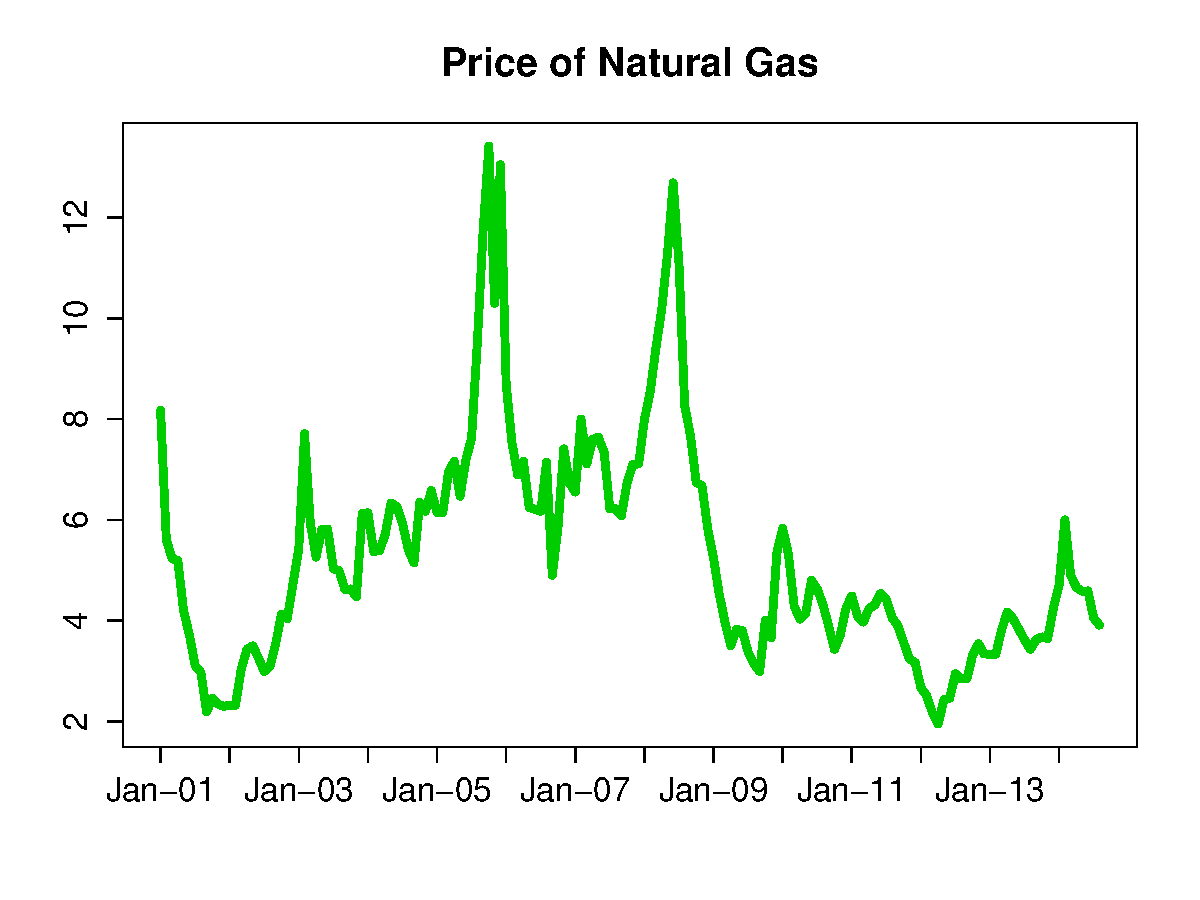
\includegraphics[width = 8cm]{PriceNG.pdf}
\end{figure}
\begin{center}
Data comes from U.S. Energy Information Administration.
\end{center}
\end{frame}

\begin{frame}
{\bf Future Prices}
\only<1>{\begin{figure}[hbt]
  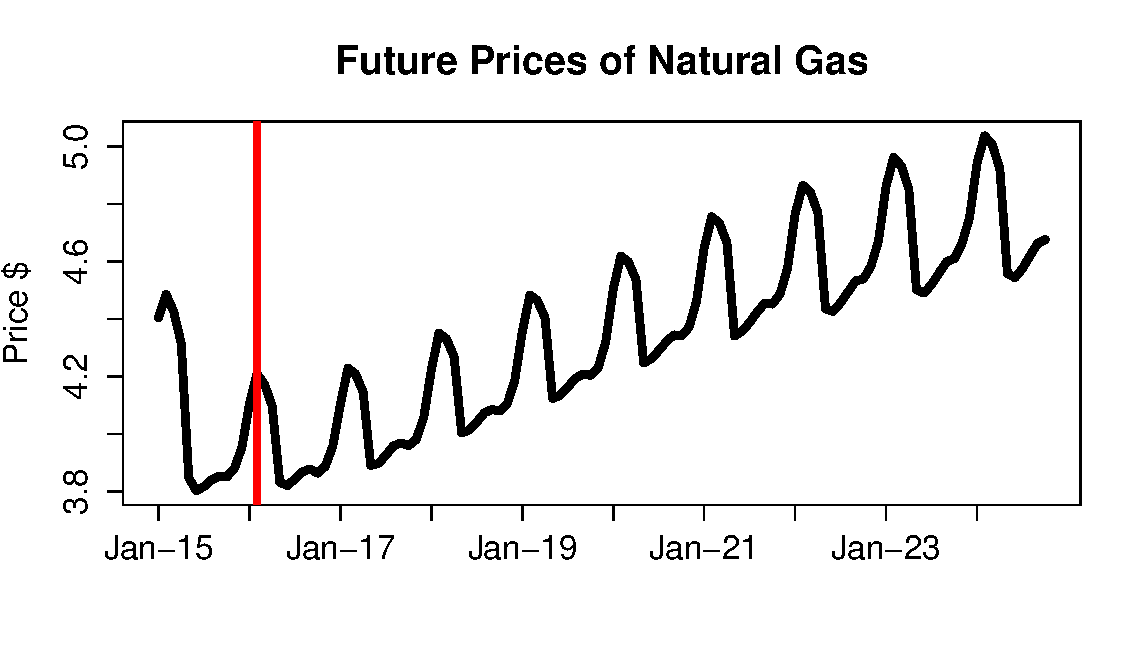
\includegraphics[width = 8cm]{FuturePrices.pdf}
\end{figure}}
\begin{center}
Data comes from U.S. Energy Information Administration.
\end{center}
\end{frame}

\begin{frame}
{\bf Future Prices}
\only<1>{\begin{figure}[hbt]
  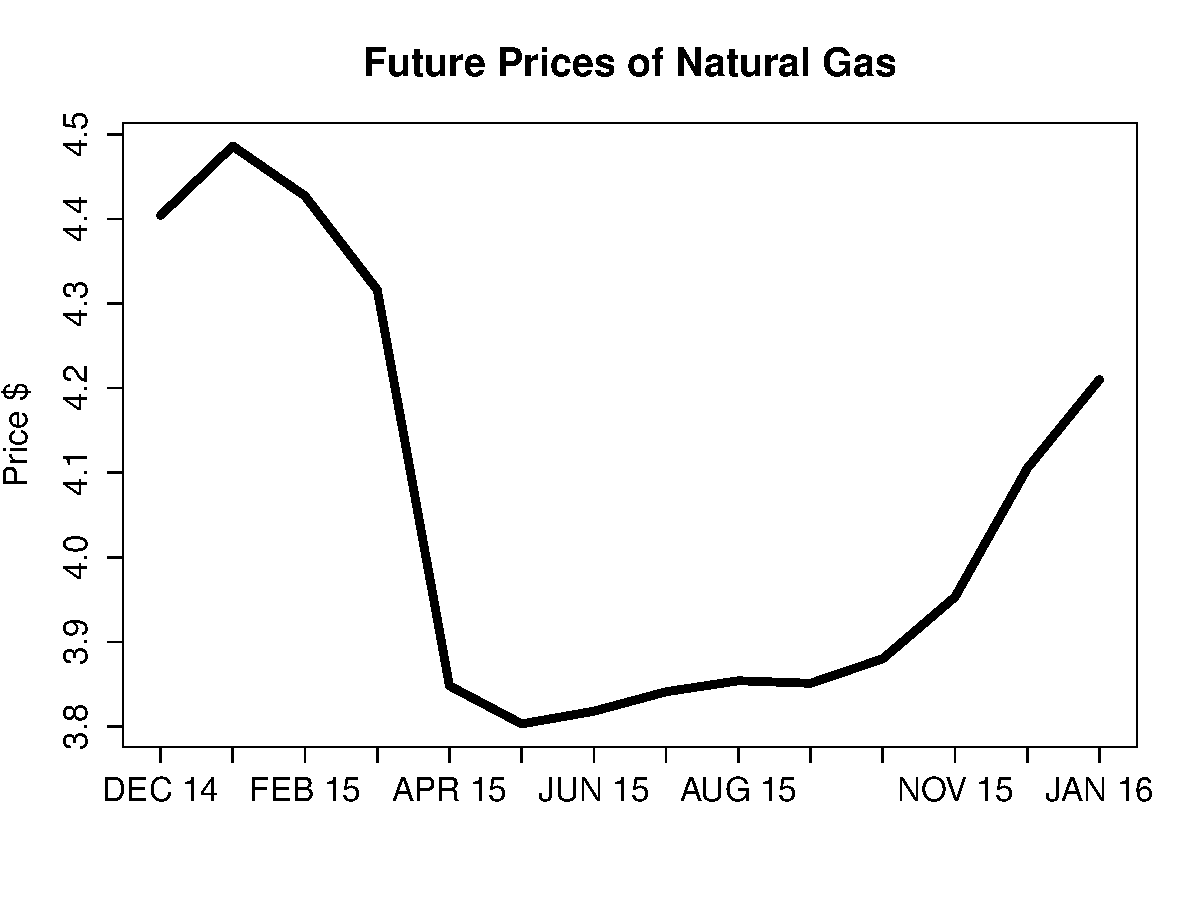
\includegraphics[width = 8cm]{FuturePrices14.pdf}
\end{figure}}
\begin{center}
Data comes from U.S. Energy Information Administration.
\end{center}
\end{frame}

\begin{frame}
{\bf Price Dynamics}

      \begin{itemize}
      \item Schwartz (1997) % The first model is a simple one-factor model in which the logarithm of the spot price of the commodity is assumed to follow a mean reverting process.
      % The second model takes into account a second stochastic factor, the convenience yield of the commodity, which is assumed to follow a mean reverting process.
      % The third model also includes stochastic interest rates.
      % For copper data, three models are of the same prediction level. For oil data, 2nd and 3rd are significantly better than the 1st.
      \item Schwartz and Smith (2000)
      %The short-Term/Long term model. Logarithm of the spot price is a mean reverting spot process with a stochastic mean. Logarithm of the spot price is decomposed into two parts short term deviations and equilibrium level. First one is OU process and the second one is a drifted brownian motion. 
      \item Routledge, Seppi and Spatt(2000)
      % Rather than exogenously assuming stochastic processes for spot prices and convenience yields, we derive the spot and forward price processes induced by a mean-reverting immediate use net- demand process and the resulting equilibrium inventory dynamics.
      \item Jaillet, Ronn and Tompaidis (2004)% seasonal factor with one factor model
      \end{itemize}
\end{frame}

\begin{frame}
{\bf Mismatch Between Production and Consumption}
\begin{figure}[hbt]
  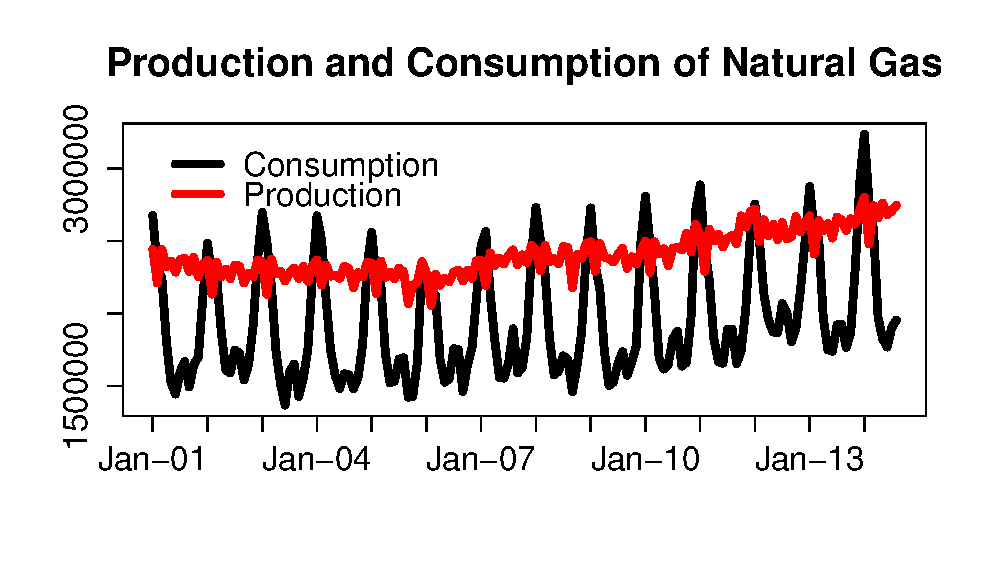
\includegraphics[width = 10cm]{DemandSupply.pdf}
\end{figure}
\begin{center}
Data comes from U.S. Energy Information Administration.
\end{center}
\end{frame}

\begin{frame}
{\bf Constraints of Storage}

\begin{itemize}
  \item Transaction costs.
  \item Depreciation.
  \item Limited delivery rate.
  \item Finite capacity.
\end{itemize}

\end{frame}




\begin{frame}
{\bf Storage Valuation}
\begin{itemize}
   \item Fackler and Livingston (2002)
  \item Hodges (2004)
  \item Chen and Forsyth (2008,2010)
  \item Boogert and Jong (2008)
  \item Thompson, Davison and Rasmussen (2009)
  \item Secomandi (2010)
\end{itemize}
\end{frame}

%%------------------------------------------------
%
\begin{frame}
{\bf Method}
\begin{itemize}
  \item Continuous Time Singular Control $\Rightarrow$ 2-d HJB equation.\\
  \item HJB equation (free boundary problem) is very hard to solve.\\
  \item Moving boundary method is used in 1 dimension.\\
  \begin{itemize}
  \item Start with an initial guess and iteratively improve it until convergence.\\
  \item A sequence of fixed boundary problems $\rightarrow$ free boundary problem\\
\end{itemize}
\end{itemize}
\end{frame}




%
\begin{frame}
{\bf 1 Dimension VS 2 Dimensions}
%Todo: give plots show that 1 dimension is way easier than 2 dimension.
\begin{columns}
   \column{0.5\textwidth}

   \begin{figure}[hbt]
   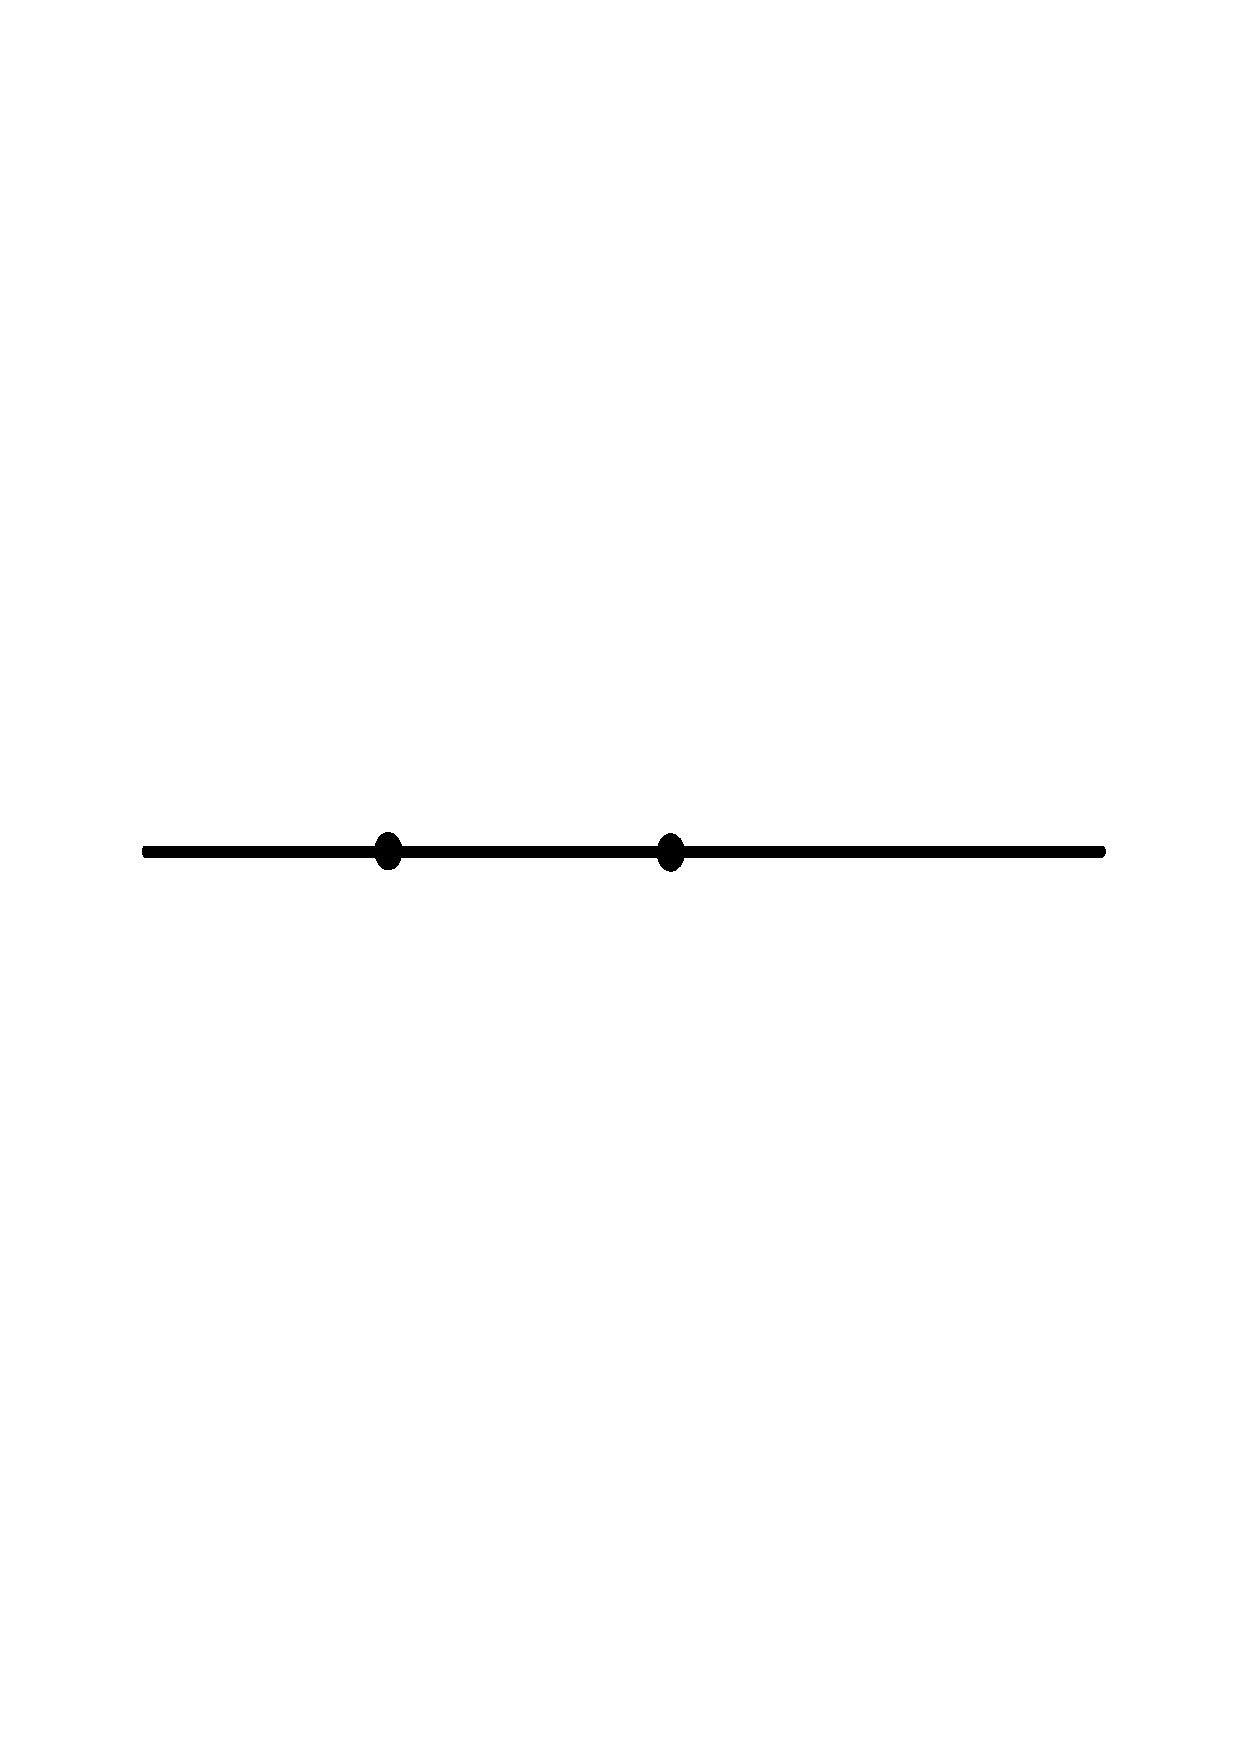
\includegraphics[width = 5cm]{1D.pdf}
   \caption{1 Dimension}
   \end{figure}
 
  \column{0.5\textwidth} 
  \begin{figure}[hbt]
  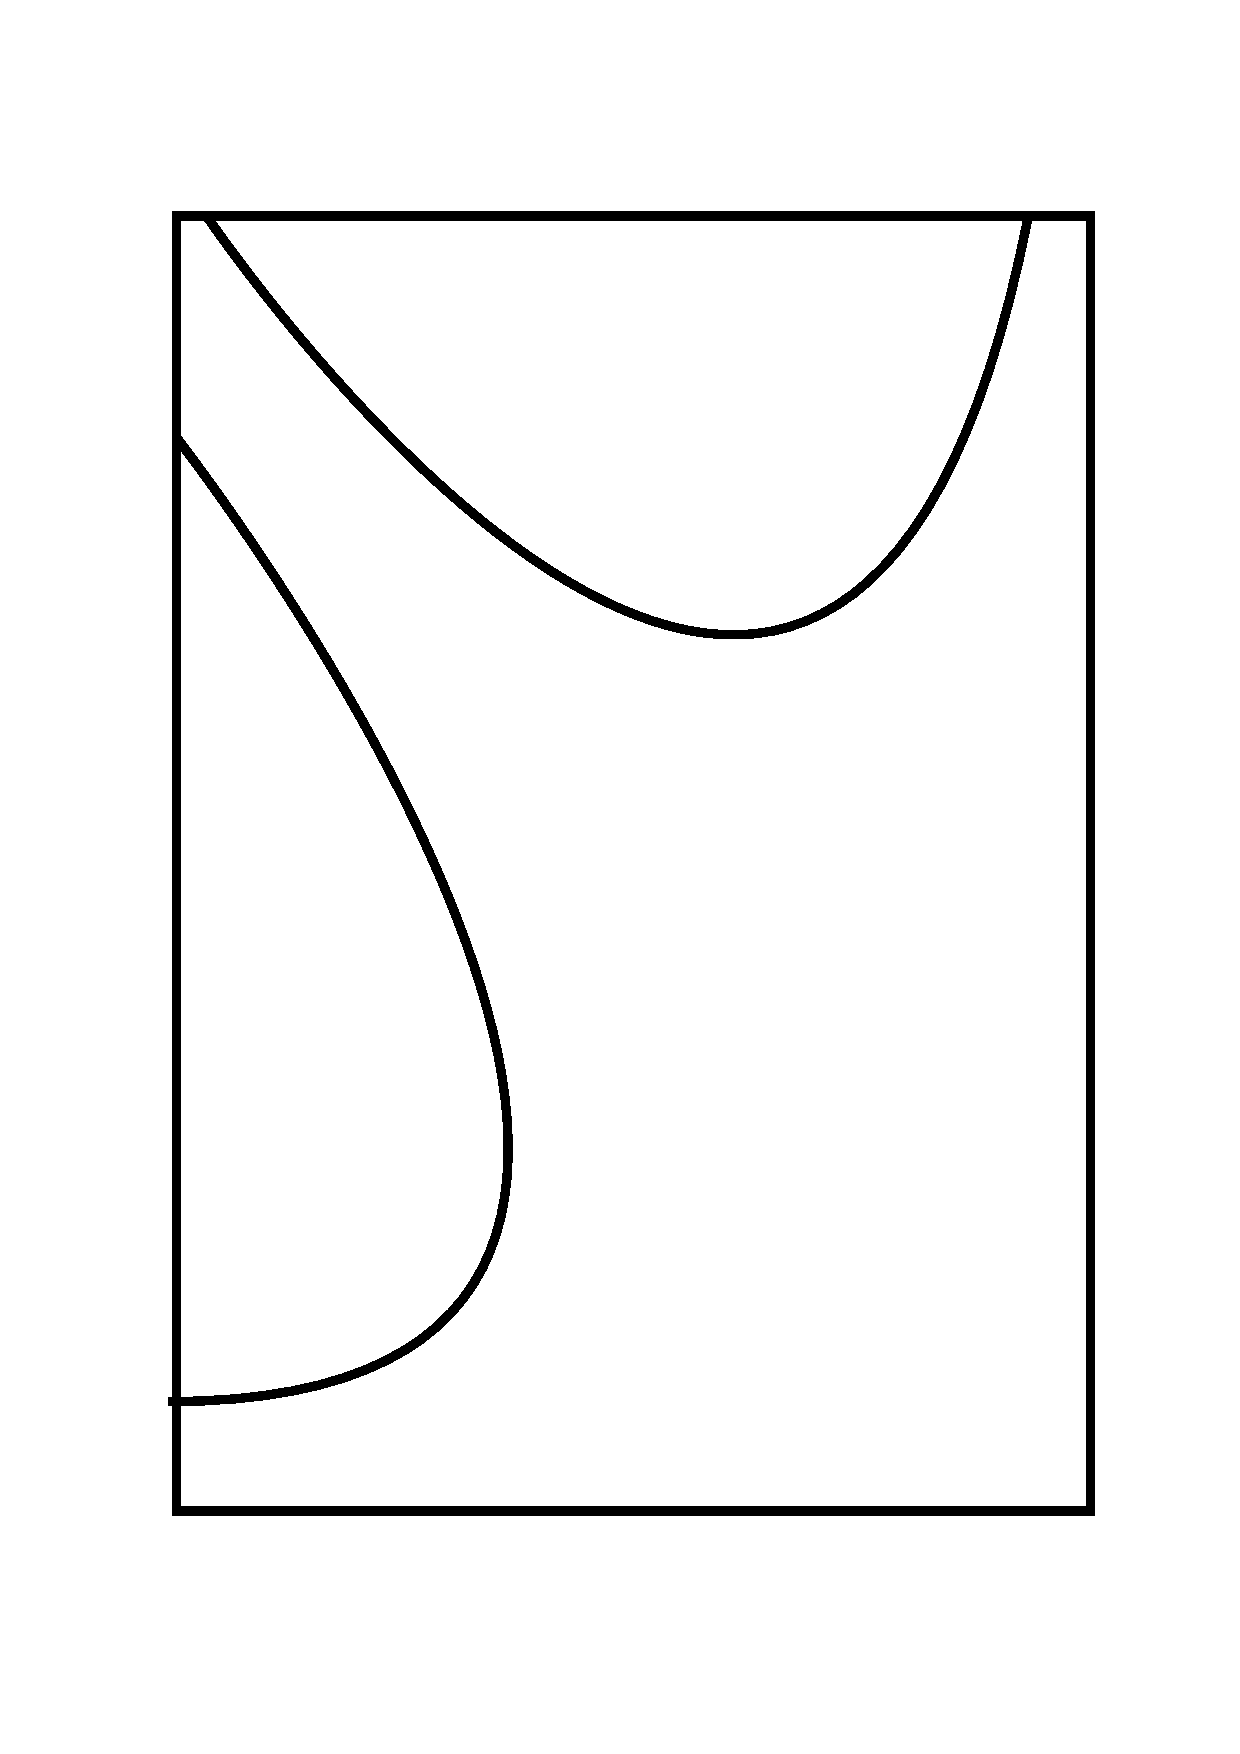
\includegraphics[width = 5cm]{2D1.pdf}
  \caption{2 Dimensions}
  \end{figure}
\end{columns}

\end{frame}

\begin{frame}
{\bf Moving Boundary Method}

\begin{itemize}
  \item Muthuraman and Kumar (2006)
  \item Chockalingam and Muthuraman (2007,2010)
  \item Muthuraman and Zha (2008)
  \item Feng and Muthuraman (2010)
\end{itemize}
\end{frame}




\begin{frame}
{\bf Overview of Results}
\begin{itemize}
\item Methodology.
\begin{itemize}
\item Fixed boundary problem is solved efficiently. 
  \item Moving boundary method is generalized to 2 dimensions.
\end{itemize}

\item Value of storage.

\begin{itemize}
  \item The value of storage with non-trivial transaction costs and finite capacity is calculated.
  \item  The optimal strategy is found.
\end{itemize}

  
%  \begin{itemize}
%  \item Initial guess.
%  \item Direction and distance of movement.
%  \item The Convergence.
%\end{itemize}
\end{itemize}

\end{frame}


\section{Model}
\begin{frame}
{\bf Model}
\begin{itemize}
  \item One factor model
\begin{equation*}
  dS_t = \kappa ( \mu - \ln S_t)S_t dt + \sigma S_t dW_t
\end{equation*}
\item By Ito's formula, $X_t = \ln(S_t)$ is an Ornstein-Uhlenbeck process,

\begin{equation*}
  dX_t = \kappa ( \alpha - X_t) dt + \sigma dW_t.
\end{equation*}

where $\alpha  = \mu - \sigma^2/(2\kappa)$.
\end{itemize}

\end{frame}

\begin{frame}
{\bf Model}
\begin{itemize}
\item Storage level at time $t$ is $Q_t$. $L_t,U_t$ represent cumulative injections and withdrawals at time $t$.

\begin{equation*}
  dQ_t = dL_t - dU_t
\end{equation*}
\\
\item Admissible if $Q_t \in (Q_{min},Q_{max})~~ \forall t \geq 0$.

\item Costs of injection and withdrawal, $\lambda(q)$ and $\mu(q)$, are monotone and bounded.

%In the natural gas example, X_t: leak or use it as the energy for pump. Q_t difficulty.
\end{itemize}

\end{frame}


\begin{frame}
{\bf Model}
\begin{itemize}
  \item Objective: to maximize discounted infinite-horizon cash flows.

  \begin{equation}
  \begin{split}
  V(x,q) &= \max_{(L,U) \in \mathcal{U}} \mathbb{E}_{x,q} \left(\int_{0}^{\infty} e^{-\beta t}(e^{X_t} - \mu(Q^{(1)}_t))dU_t\right.\\
  &\left.- \int_{0}^{\infty}e^{-\beta t}(e^{X_t} + \lambda(Q^{(2)}_t))dL_t\right)
  \end{split}
\end{equation}
% I need to mention this.
where $X_0 =x$ and $Q_0 = q$. %What's more,
%\begin{equation}
%\begin{split}
%  \mu(Q^1_t) = \frac{1}{U_t - U_{t-}}\int_{U_{t-}}^{U_t} \mu(q) dq
%  \end{split}
%\end{equation}
%
%\begin{equation}
%  \lambda(Q^2_t) = \frac{1}{L_t - L_{t-}}\int_{L_{t-}}^{L_t} \lambda(q) dq.
%\end{equation}  
  
\end{itemize}
\end{frame}

\begin{frame}
{\bf $\mu = 0,~ \lambda = 0$ and $\beta = 0$}
\only<1>{
\begin{figure}[hbt]
  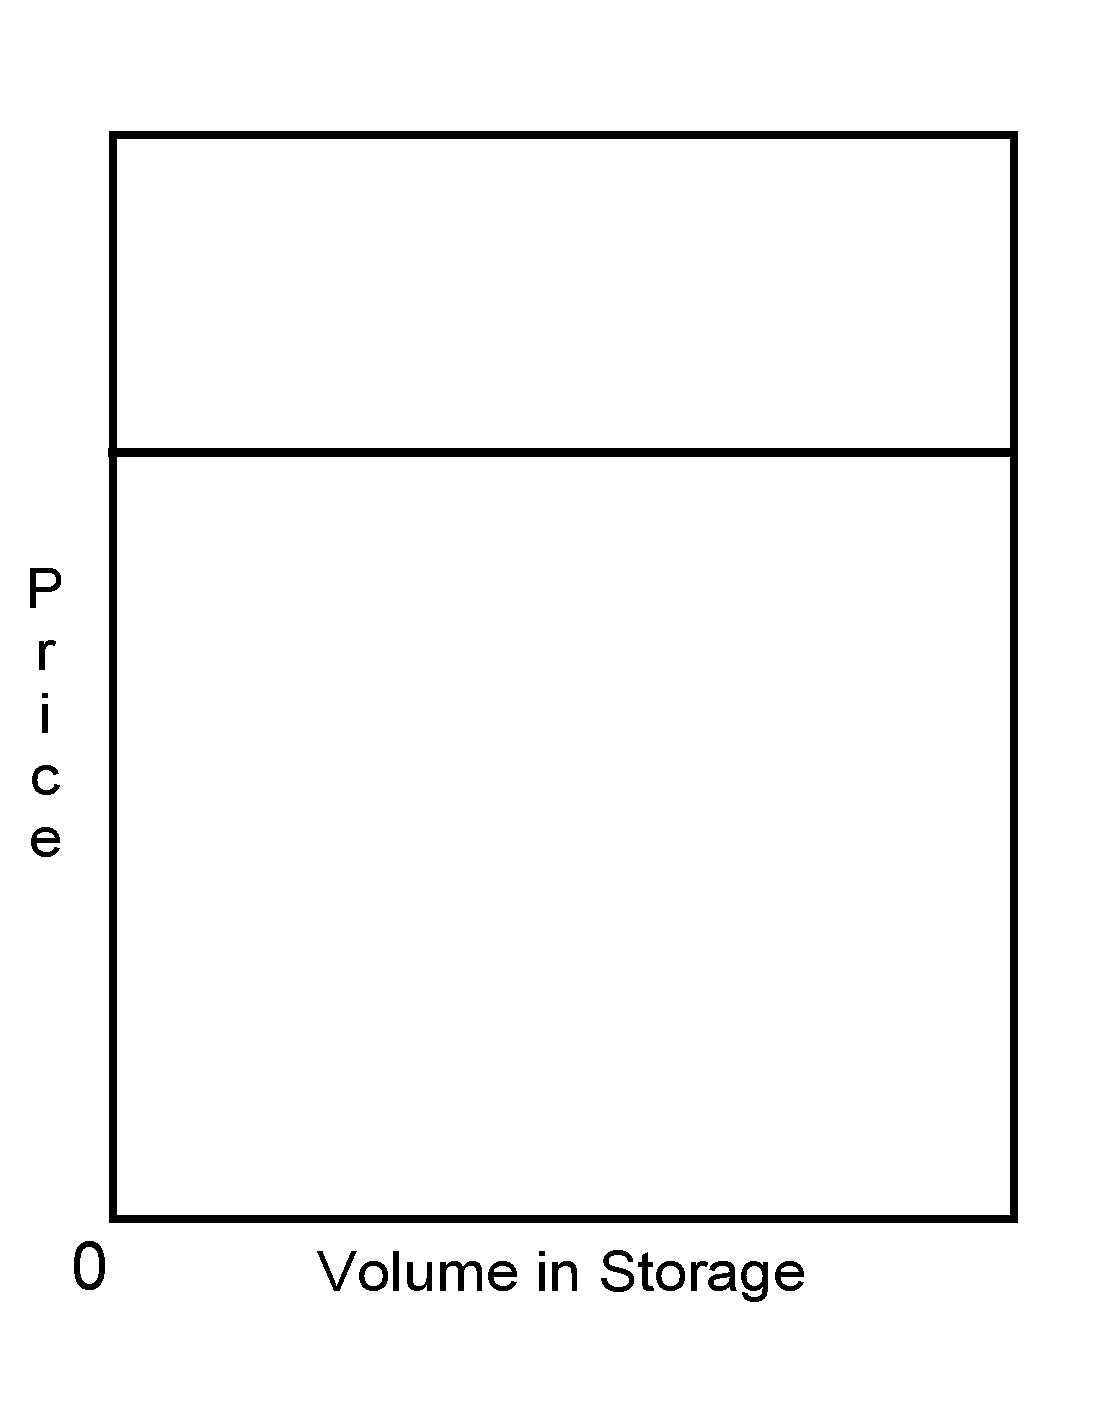
\includegraphics[scale= 0.25]{NonCostBeta01.pdf}
\end{figure}
}

\only<2>{
\begin{figure}[hbt]
  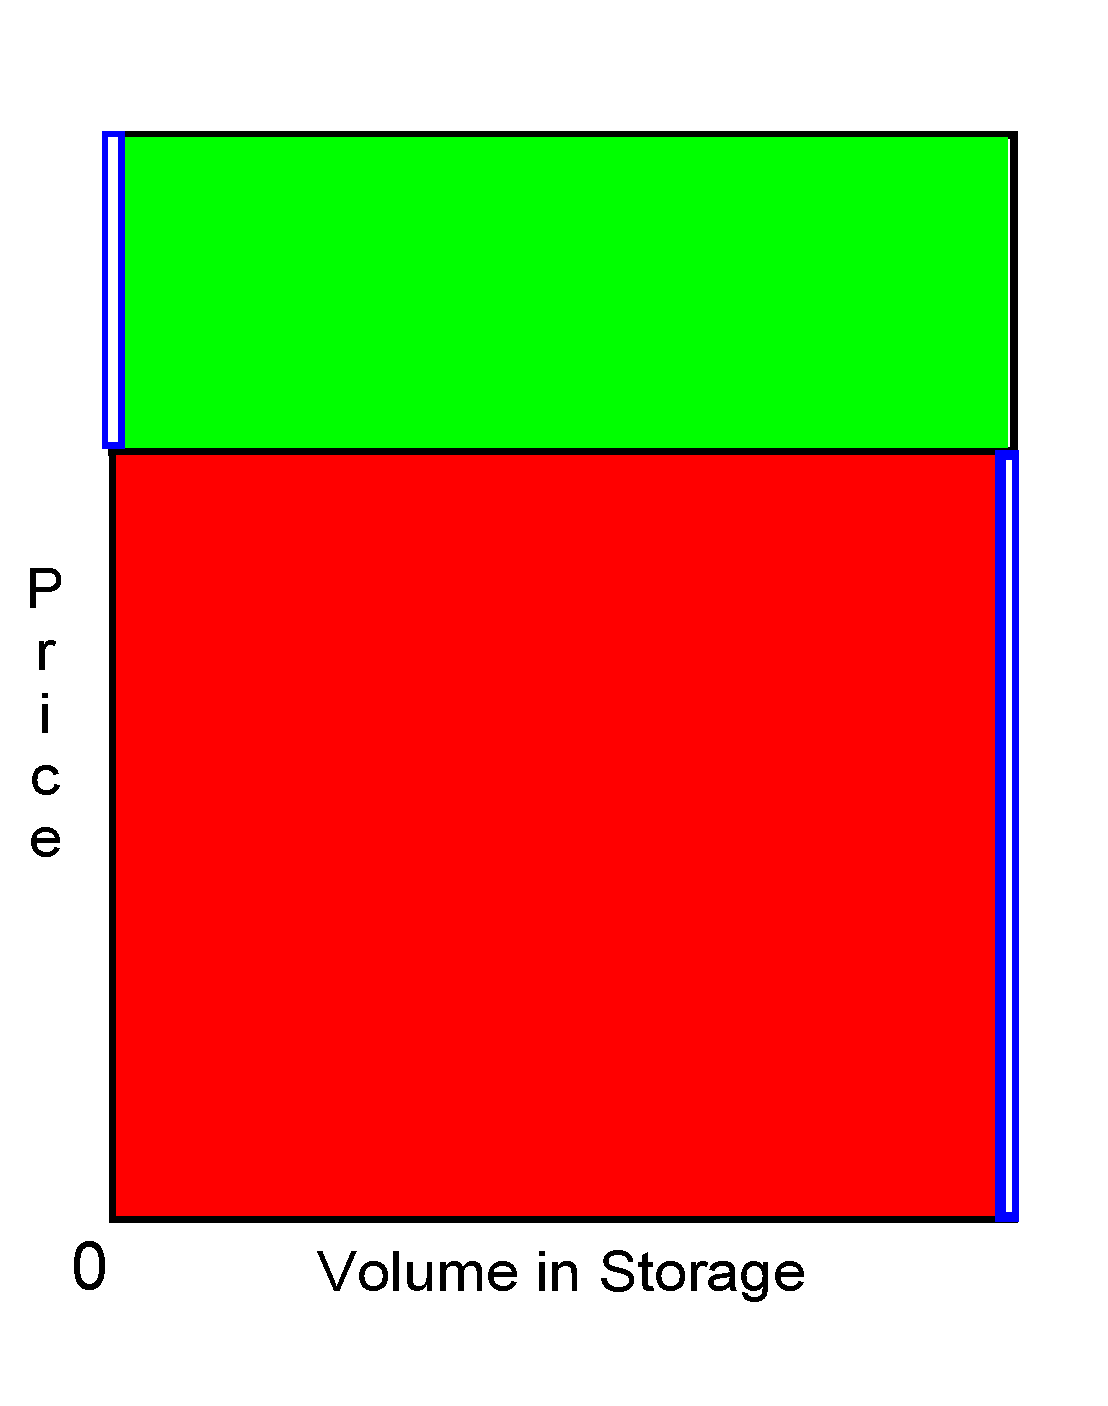
\includegraphics[scale= 0.25]{NonCostBeta02.pdf}
\end{figure}
}
\end{frame}

\begin{frame}
{\bf  $\mu = 0,~ \lambda = 0$ but $\beta > 0$}
\begin{figure}[hbt]
  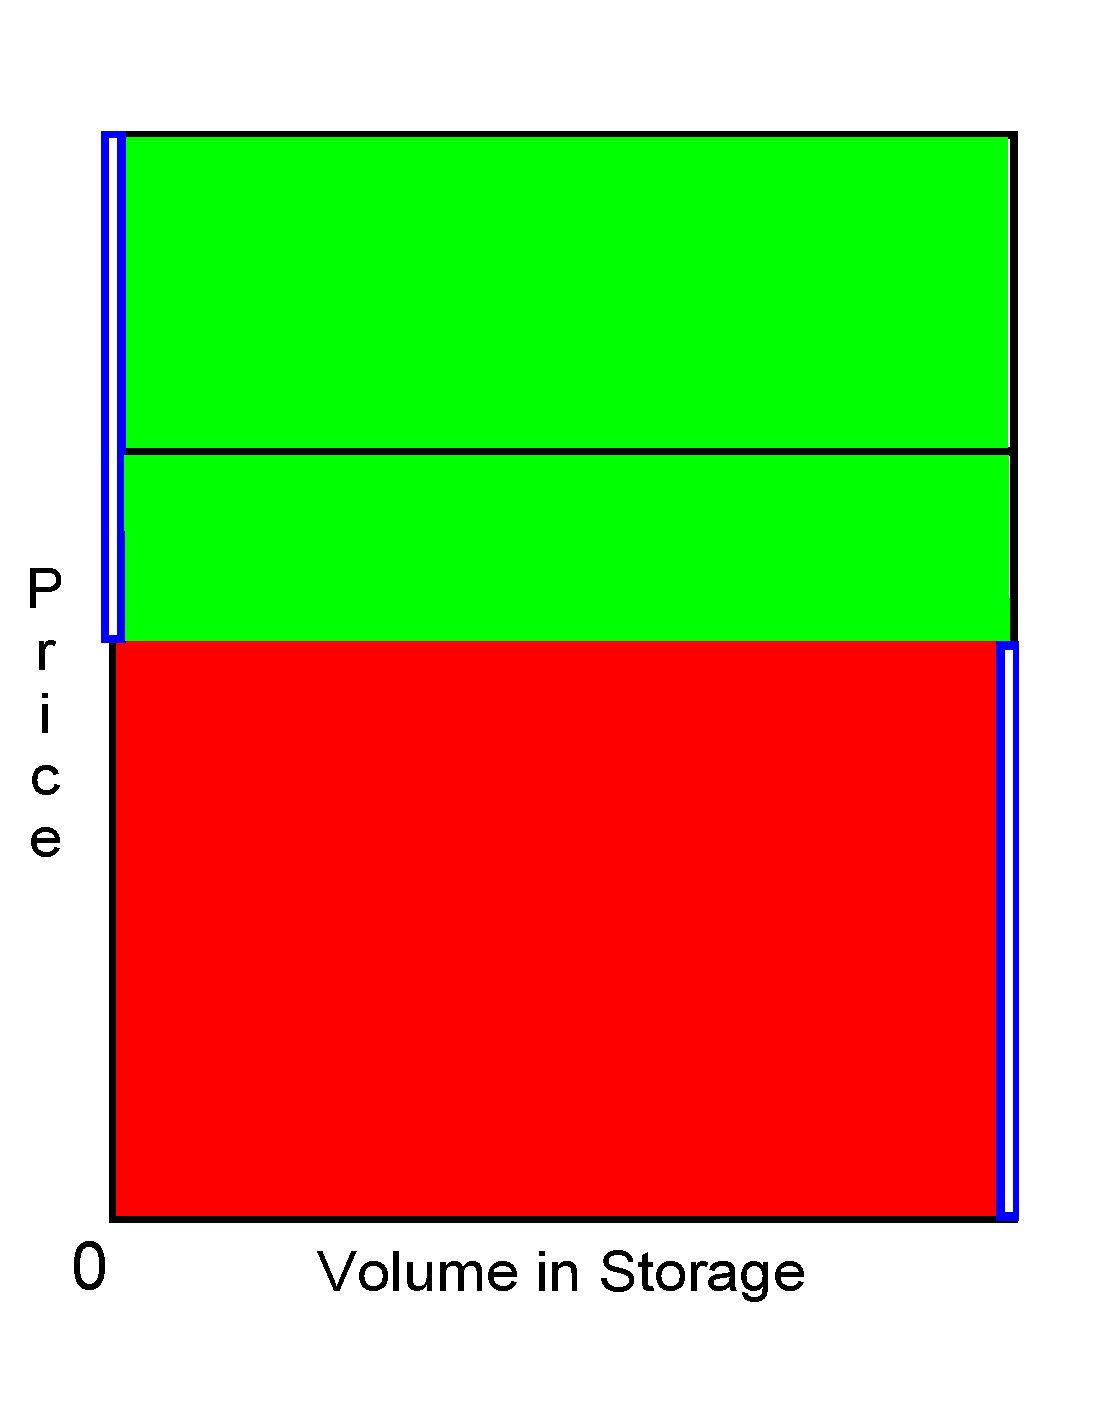
\includegraphics[scale= 0.25]{NonCostBetaNot0.pdf}
\end{figure}
\end{frame}

\begin{frame}
{\bf $\mu = \text{Constant}>0,~ \lambda = \text{Constant}>0$ and $\beta > 0$}

\begin{columns}
  \column{0.5\textwidth}
  \only<1-2>{
\begin{figure}[hbt]
  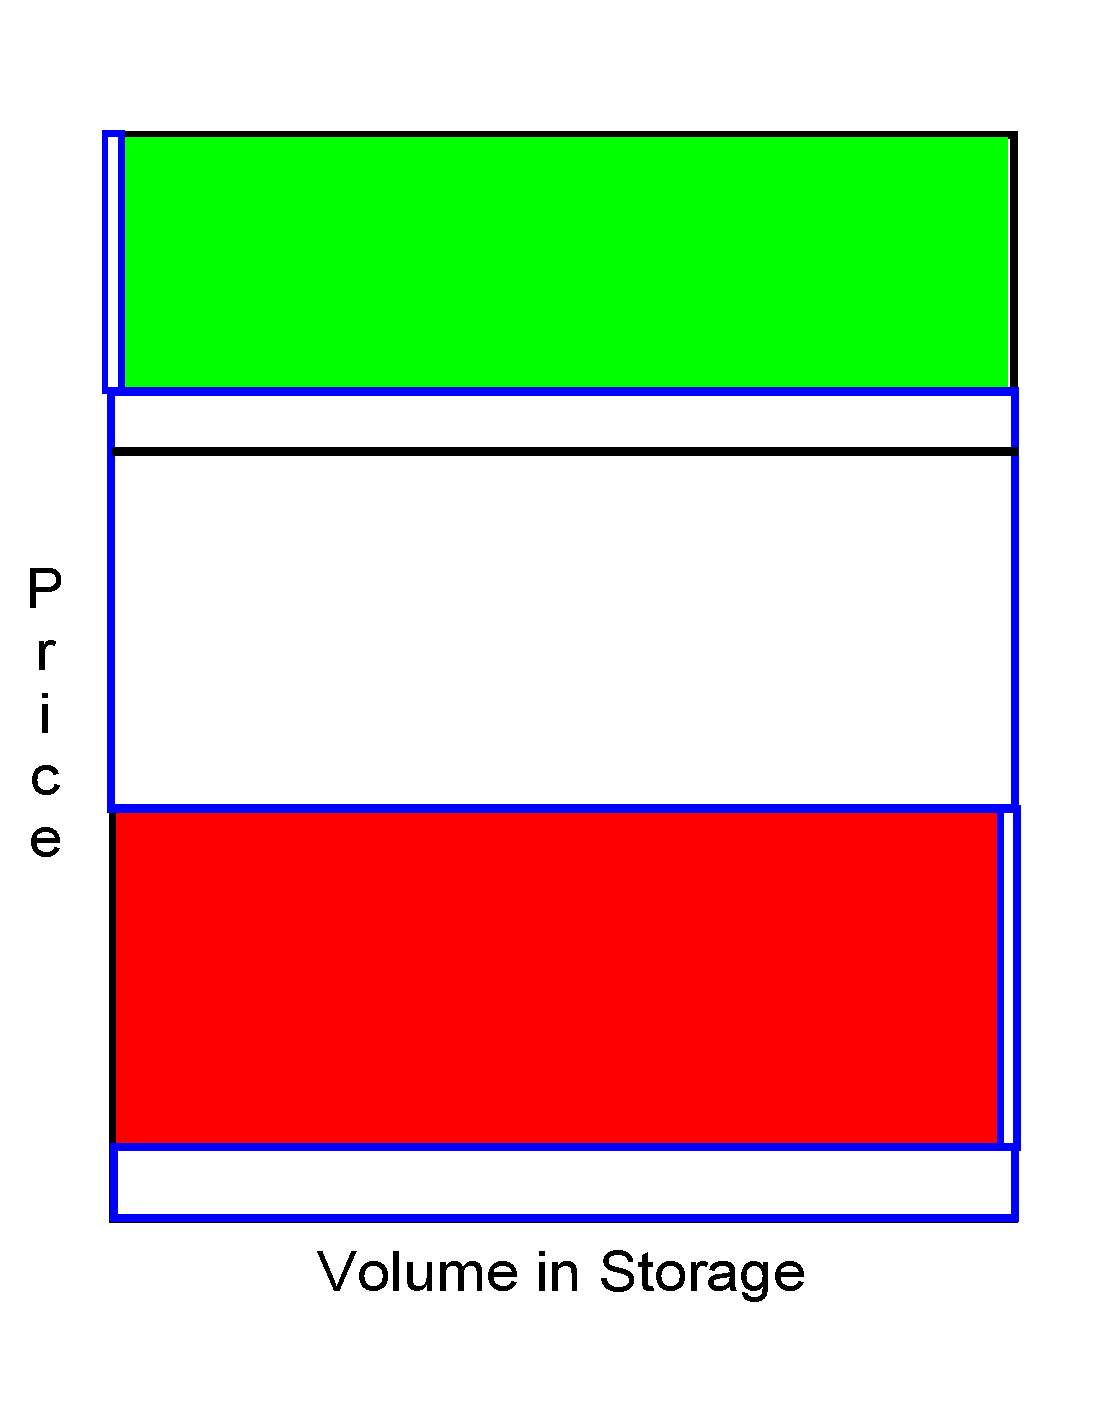
\includegraphics[scale= 0.25]{ConstCostBetaNot0.pdf}
\end{figure}
}

\only<3>{
\begin{figure}[hbt]
  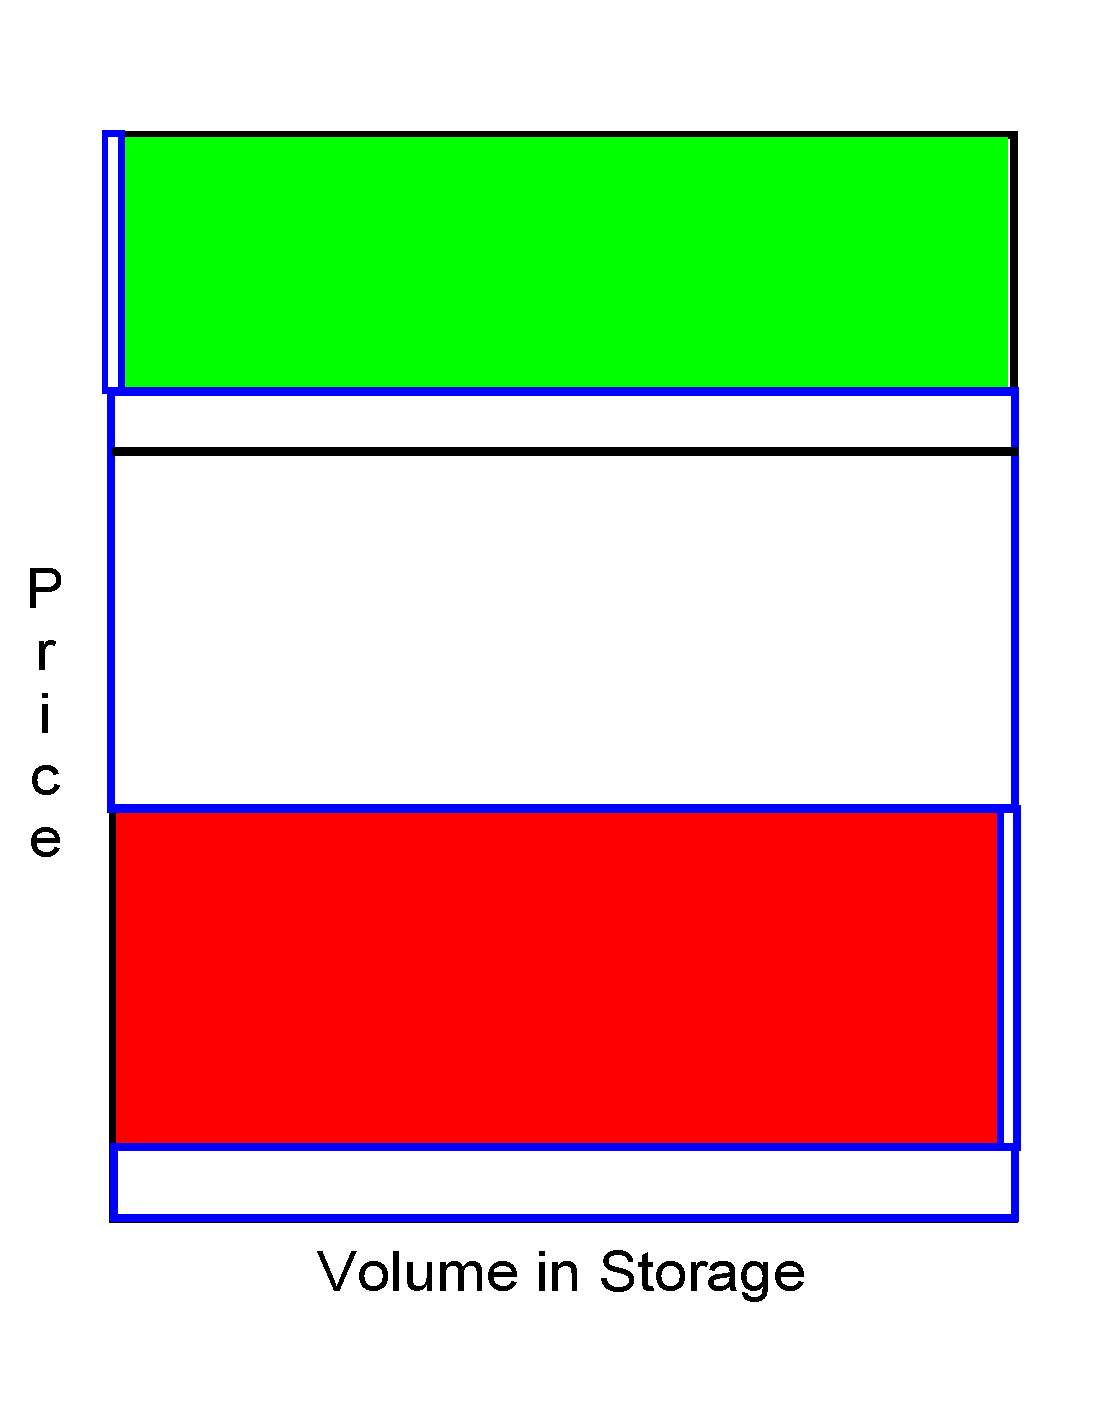
\includegraphics[scale= 0.25]{ConstCostBetaNot0.pdf}
  \caption{Small $\lambda$}
\end{figure}

}
  \column{0.5\textwidth}
  \only<1>{ 
\begin{figure}[hbt]
  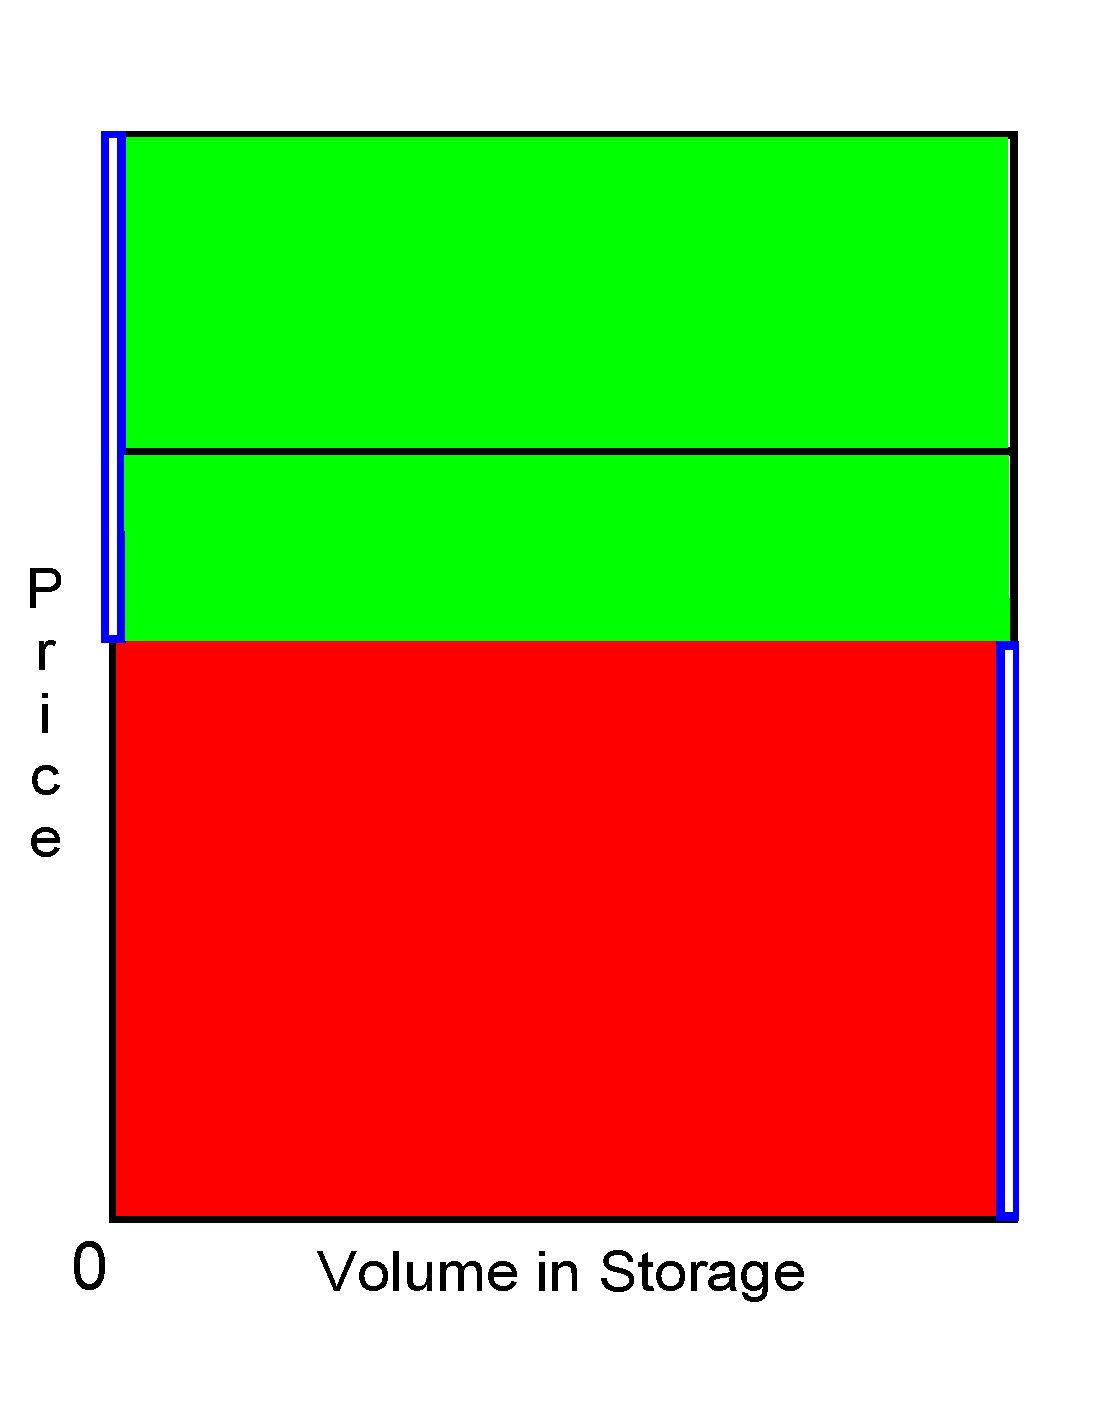
\includegraphics[scale= 0.25]{NonCostBetaNot0.pdf}
\end{figure}
}
\only<2>{
\begin{equation*}
 V(s) = \sup_{\tau \in \mathcal{T}}\mathbb{E}_s\{e^{-\beta \tau} \left(S_\tau - \mu\right)\} 
\end{equation*}

$V(0+) = 0$\\

If $V(s) - (s + \lambda) < 0$, do not buy at Price $s$.\\

$V(0+) - (0 + \lambda) = -\lambda < 0$.\\

}


\only<3>{
\begin{figure}[hbt]
  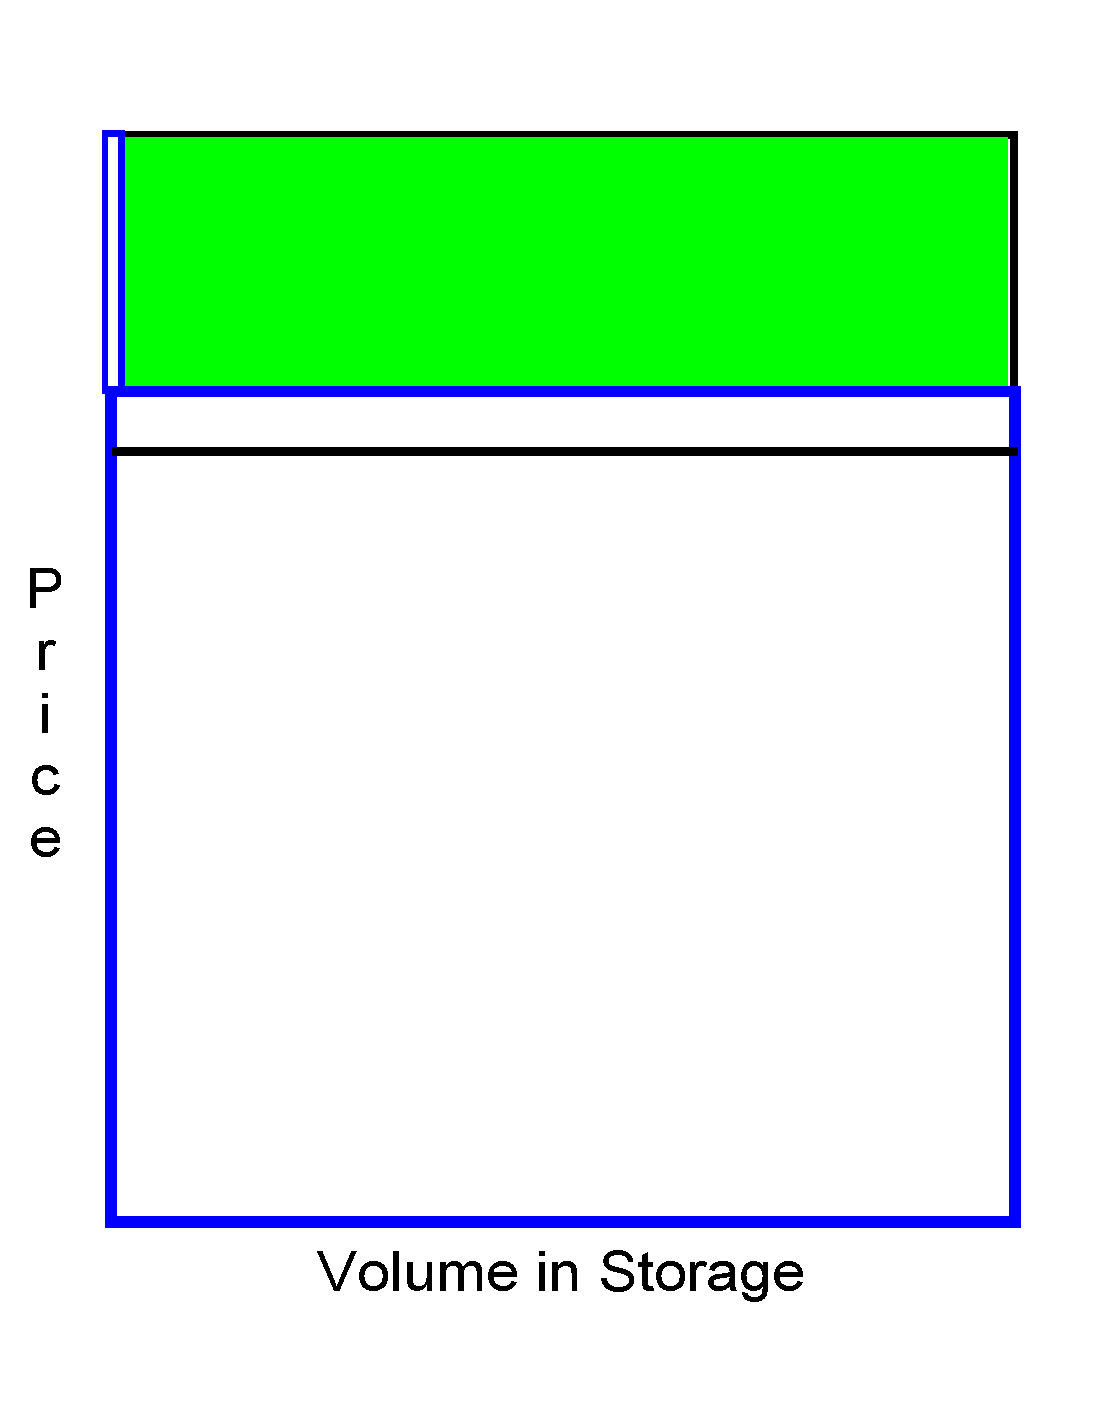
\includegraphics[scale= 0.25]{ConstCostBetaNot0Case2.pdf}
  \caption{Large $\lambda$}
\end{figure}
}
\end{columns}

\end{frame}

\begin{frame}
{\bf Observation}

\begin{block}{Observation}
When the price is high enough, regardless of storage, selling is the optimal strategy.
\end{block}

%   \begin{block}{Observation 2}
%At the same price level, selling and buying can't be both optimal.
%    \end{block}

\end{frame}



\begin{frame}
{\bf $\mu(q) \downarrow,~ \lambda(q) \uparrow$ and $\beta > 0$}

\begin{figure}[hbt]
  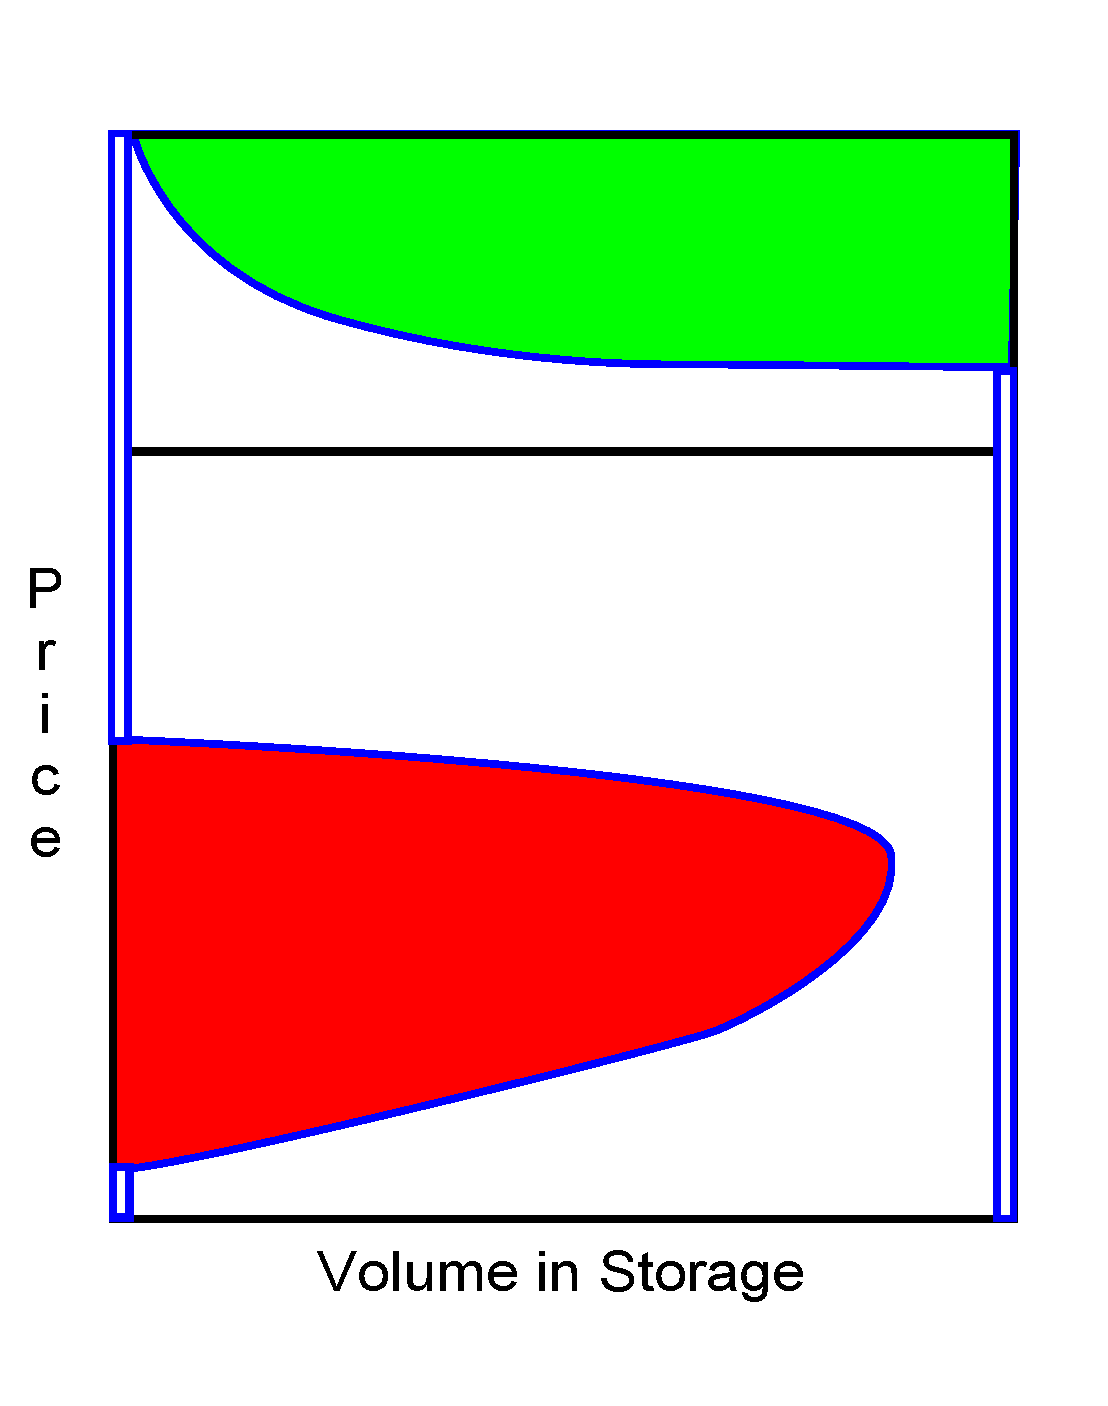
\includegraphics[scale= 0.25]{NotConstCostBetaNot0.pdf}
\end{figure}


\end{frame}





\begin{frame}
{\bf The Hamilton-Jacobi-Bellman Equation}
\begin{itemize}
  \item Dynamic programming arguments and Ito's formula yield the Hamilton-Jacobi-Bellman (HJB) equation.
  \begin{equation*}
  \max\left( \mathcal{L} V, \frac{\partial V}{\partial q} - (e^x + \lambda(q)), -\frac{\partial V}{\partial q} + (e^x - \mu(q))\right) = 0
\end{equation*}
with $\mathcal{L}V = \frac{1}{2} \sigma^2 \frac{\partial^2 V}{\partial x^2} + \alpha (\kappa - x) \frac{\partial V}{\partial x} - \beta V$.


  \item A verification theorem assures us that a function that solves the HJB equation is the value function for the original control problem and a policy that achieves this value function is the optimal policy.

\end{itemize}

\end{frame}

\begin{frame}
{\bf The Hamilton-Jacobi-Bellman Equation}
%The first part is the discounted value earned in the future while the second part is the cost I need to pay right now.

\begin{itemize}
\item Assume $V$ is known and the change of policy at one point $(x_0,q_0)$ won't affect it.\\
Now at $(x_0,q_0)$, $\epsilon$ is bought at price $e^{x_0}$. The average buying profit is 
\begin{equation*}
  \frac{\left[V(x_0,q_0 + \epsilon) - V(x_0,q_0)\right] - \epsilon(e^x + \lambda(q))}{\epsilon}
  \stackrel{\epsilon \rightarrow 0}{\longrightarrow} 
  \frac{\partial V}{\partial q} - (e^x + \lambda(q))
\end{equation*}

\item $\mathcal{L}V(x,q)$: holding profit at $(x,q)$.
\item $\frac{\partial V}{\partial q}(x,q) - (e^x + \lambda(q))$: buying profit at $(x,q)$.
\item $-\frac{\partial V}{\partial q}(x,q) + (e^x - \mu(q))$: selling profit at $(x,q)$.

\item HJB equation.
\begin{equation*}
  \max\left( \mathcal{L} V, \frac{\partial V}{\partial q} - (e^x + \lambda(q)), -\frac{\partial V}{\partial q} + (e^x - \mu(q))\right) = 0
\end{equation*}



\end{itemize}

\end{frame}


\begin{frame}
{\bf Holding, Selling and Buying Regions}
\only<1>{
\begin{itemize}
  \item The state space $(x,q) \in \mathbb{R}^2_+$ is divided into three kinds of regions.
  \item Holding region: holding profit = 0, selling \& buying profit $<0$
  \item Selling region: selling profit = 0, holding \& buying profit $<0$ 
  \item Buying region: buying profit = 0, holding \& selling profit $<0$
\end{itemize}
}

\end{frame}

\begin{frame}
{\bf Solving the Fixed Boundary Problem}
\begin{itemize}
  \item In the holding region
  \begin{equation*}
  \frac{1}{2} \sigma^2 \frac{\partial^2 V}{\partial x^2} + \alpha (\kappa - x) \frac{\partial V}{\partial x} - \beta V = 0
\end{equation*}

\item Defining $y = \kappa (x-\alpha)^2/\sigma^2$, we have
\begin{equation*}
  y \frac{\partial^2 V}{\partial y^2} + (0.5 - y) \frac{\partial V}{\partial y} -\frac{\beta}{2\kappa} V = 0
\end{equation*}

which is the Kummer Equation. The solution is the sum of hypergeometric1F1 and the hypergeometricU functions.

\begin{equation*}
\begin{split}
  V(x,q) &= A(q)\text{HyperGeoU}\left(\frac{\beta}{2\kappa},\frac{1}{2},\frac{\kappa}{\sigma^2}(x-\alpha)^2\right) \\
  &+ B(q)\text{HyperGeo1F1}\left(\frac{\beta}{2\kappa},\frac{1}{2},\frac{\kappa}{\sigma^2}(x-\alpha)^2\right)
  \end{split}
\end{equation*}

Boundary conditions can determine $A(q)$ and $B(q)$.

\end{itemize}

\end{frame}



\section{Moving Boundary Method}
\begin{frame}
{\bf The Moving Boundary Method}

Idea: Start with an initial guess and iteratively improve it until convergence.
\begin{columns}
   \column{0.4\textwidth} 
\begin{itemize}
  \item Challenges
  \begin{itemize}
  \item Initial guess.
  \item 2 dimensions.
\begin{itemize}
  \item Direction.
  \item Distance.
\end{itemize}
  \end{itemize}
\end{itemize}
  \column{0.7\textwidth}
  \only<2>{
  \begin{theorem}
When the price is high enough, regardless of storage, selling is the optimal strategy.
\end{theorem}
  }
\only<3>{\begin{figure}[hbt]
  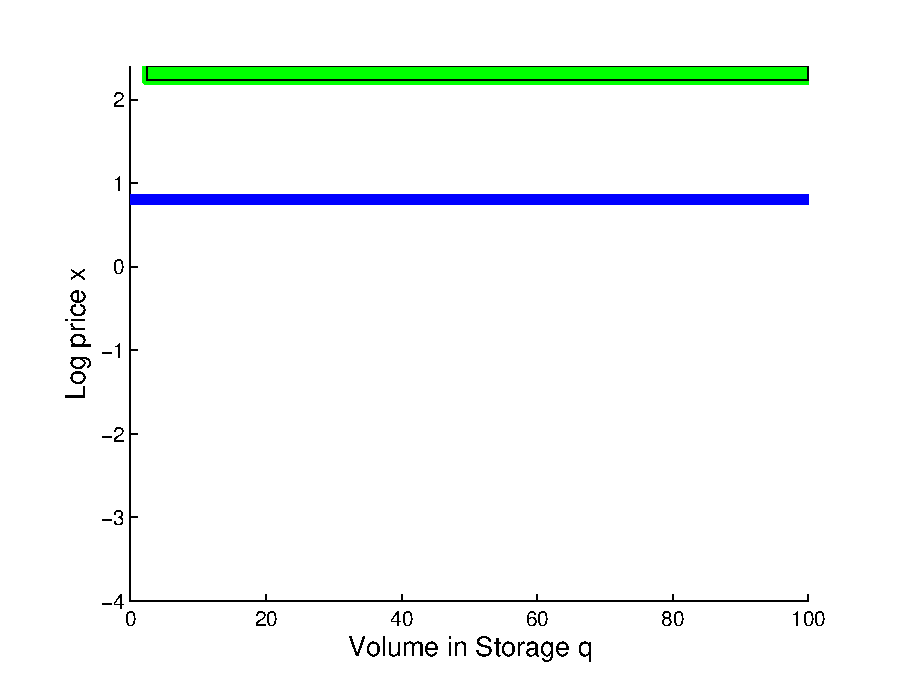
\includegraphics[scale = 0.4]{0step.eps}
  \caption{Initial Guess}
  \end{figure}}
\only<4>{\begin{figure}[hbt]
  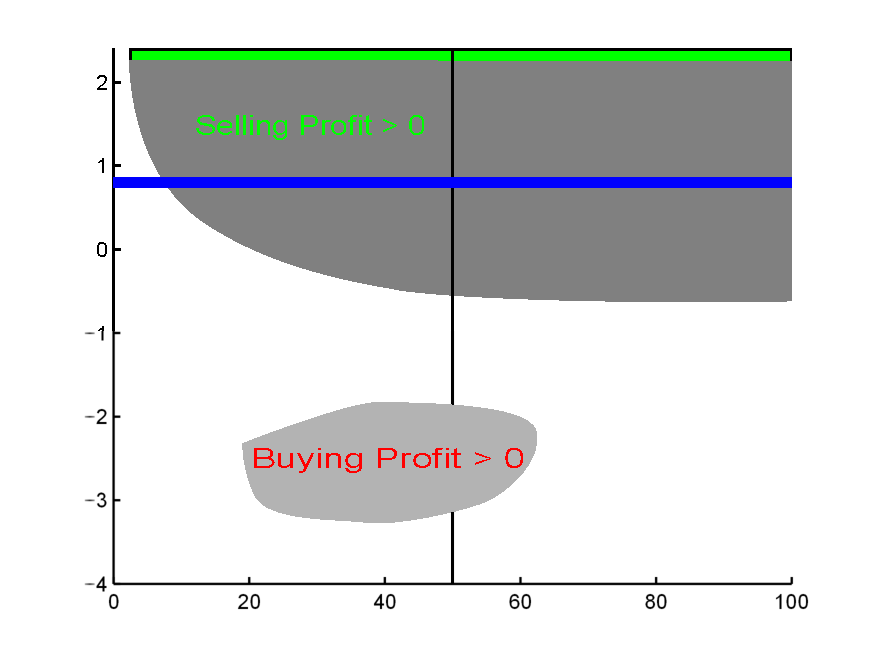
\includegraphics[scale = 0.4]{Where2Move0stepHJBViolation.pdf}
  \caption{Initial Guess}
\end{figure}}
  
  
\only<5>{\begin{figure}[hbt]
  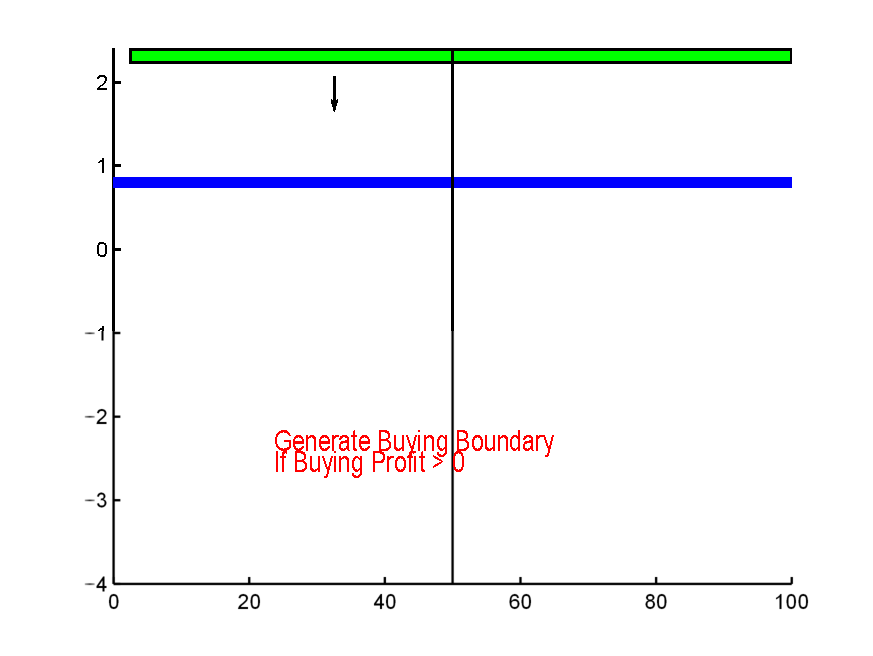
\includegraphics[scale = 0.4]{Where2Move0stepIncludingBuying.pdf}
  \caption{Initial Guess}
\end{figure}}
  \end{columns}
\end{frame}

\begin{frame}
{\bf Algorithm}
\begin{enumerate}
  \item Begin with selling at very high price for all $q>0$.
  \item Move selling and buying boundaries along price $x$ alternatively until convergence. 
%  \begin{itemize}
%  \item  The initial guess of buying is generated in this procedure.
%  \item  Each time move to the point that generates highest positive profit.
%\end{itemize}



\end{enumerate}

\end{frame}


%\begin{frame}
%{\bf How does Moving Boundary Method Work?}
%
%%todo: use movie instead of pictures to show this. At first show it extremely slow then increase the speed toward the end.
%\centering
%\only<1>{
%\begin{figure}[hbt]
%  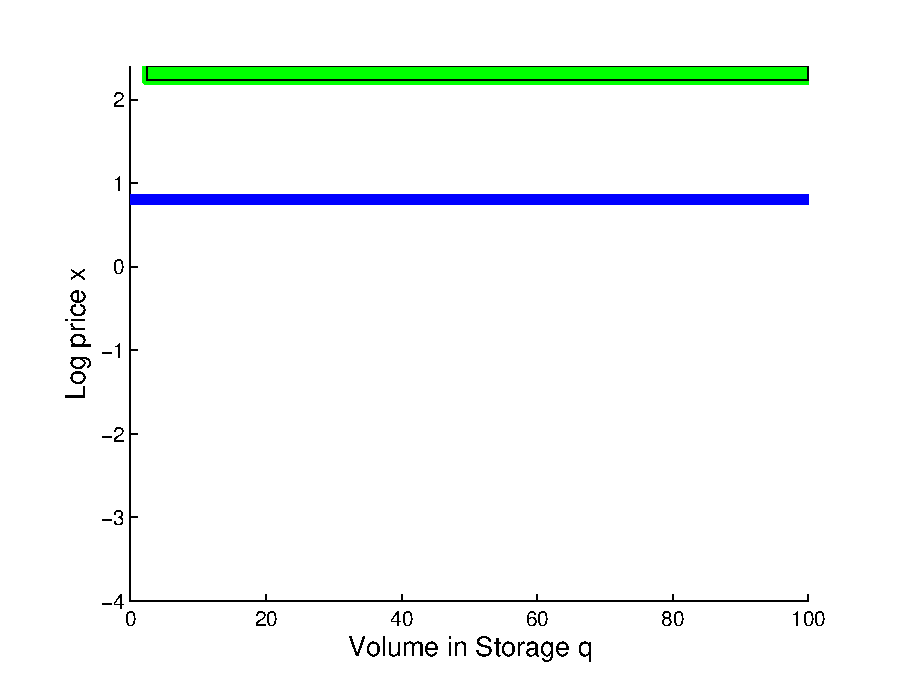
\includegraphics[scale = 0.5]{0step.eps}
%  \caption{Initial Policy}
%\end{figure}
%}
%
%%%\only<2>{
%%%\begin{figure}[hbt]
%%%  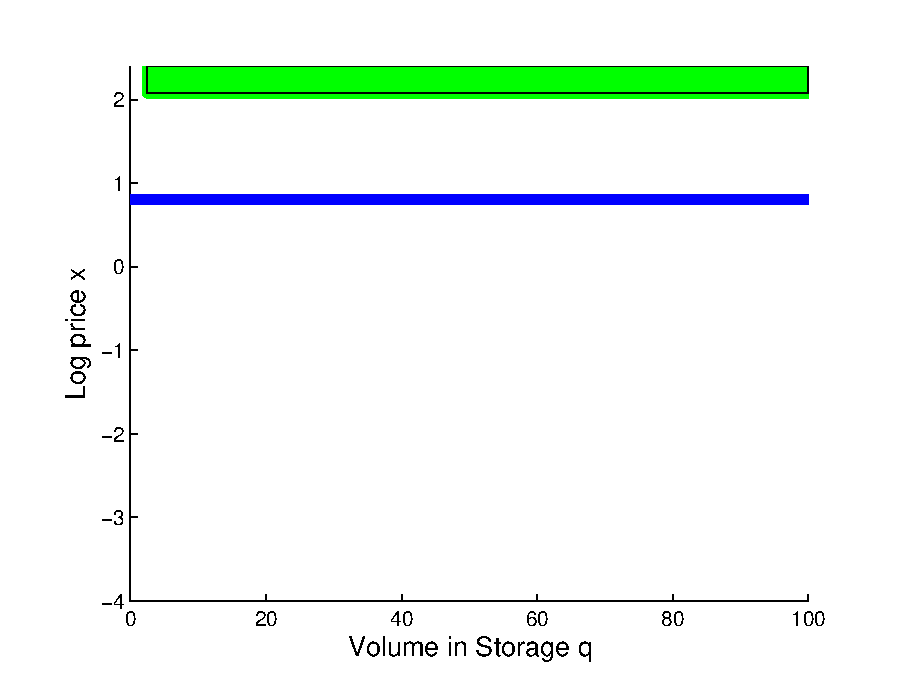
\includegraphics[scale = 0.5]{1step.eps}
%%%  \caption{1st Step}
%%%\end{figure}
%%%}
%%%\only<3>{
%%%\begin{figure}[hbt]
%%%  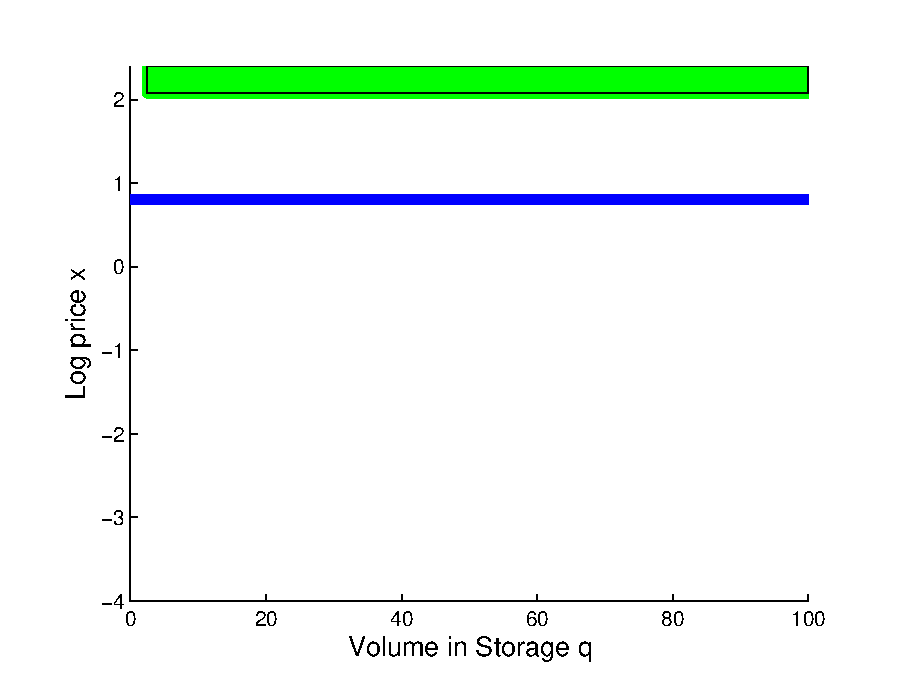
\includegraphics[scale = 0.5]{2step.eps}
%%%  \caption{2nd Step}
%%%\end{figure}
%%%}
%%%\only<4>{
%%%\begin{figure}[hbt]
%%%  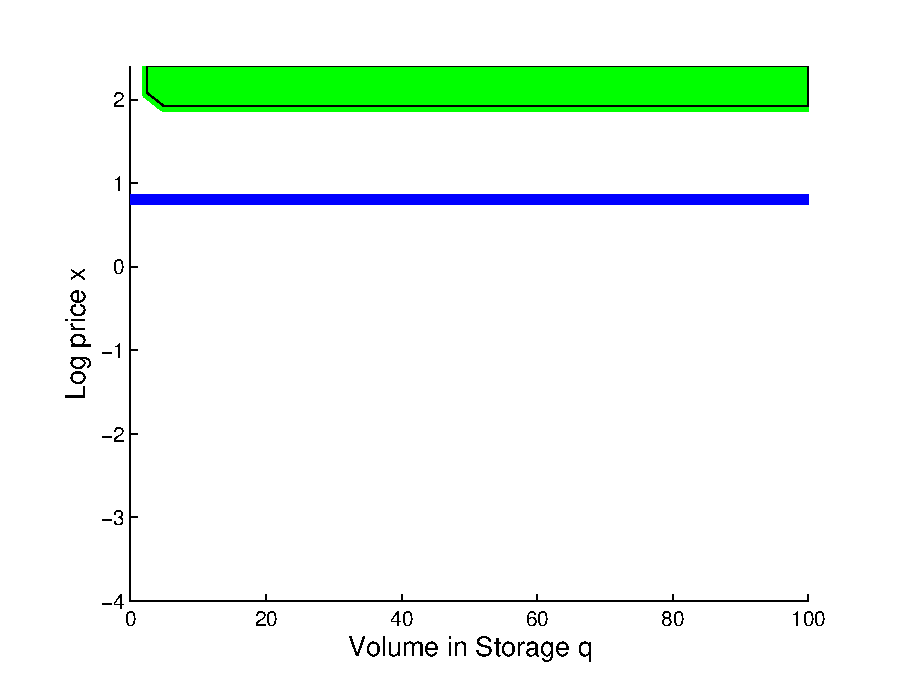
\includegraphics[scale = 0.5]{3step.eps}
%%%  \caption{3rd Step}
%%%\end{figure}
%%%}
%
%\only<2>{
%\begin{figure}[hbt]
%  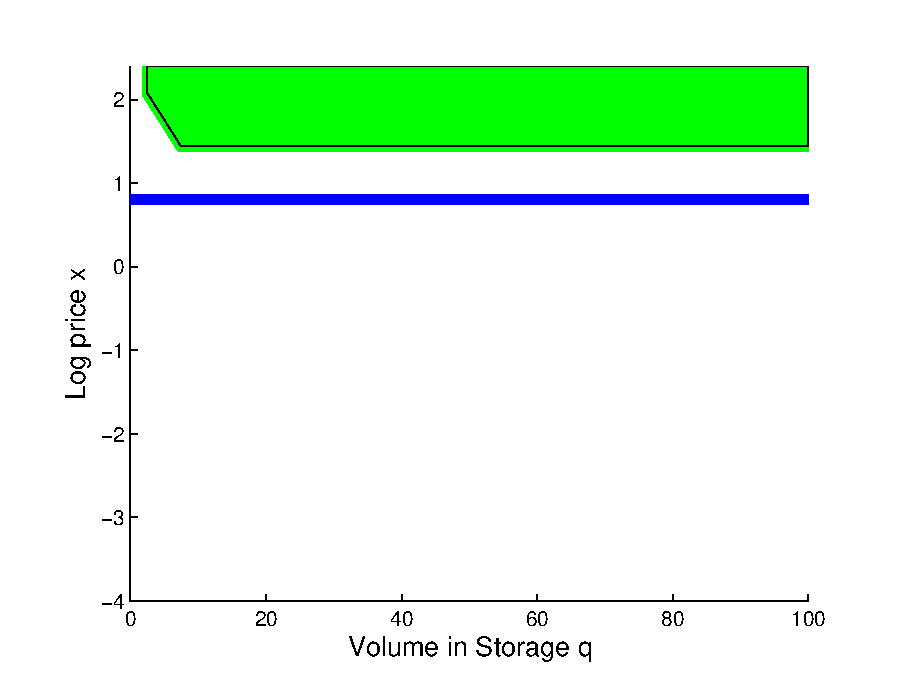
\includegraphics[scale = 0.5]{9step.eps}
%  \caption{9th Step}
%\end{figure}
%}
%
%\only<3>{
%\begin{figure}[hbt]
%  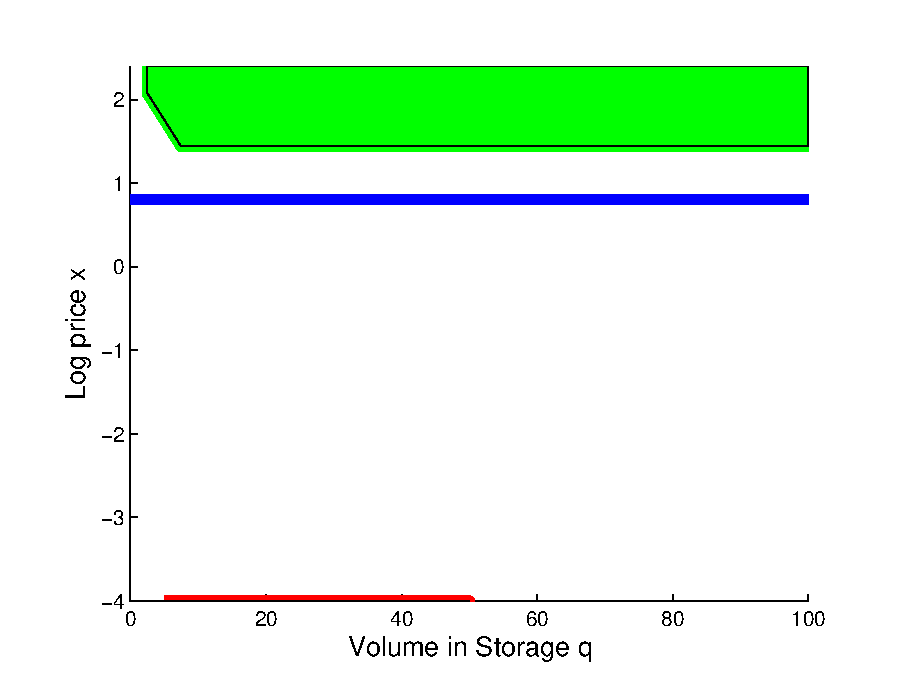
\includegraphics[scale = 0.5]{10step.eps}
%  \caption{10th Step}
%\end{figure}
%}
%
%\only<4>{
%\begin{figure}[hbt]
%  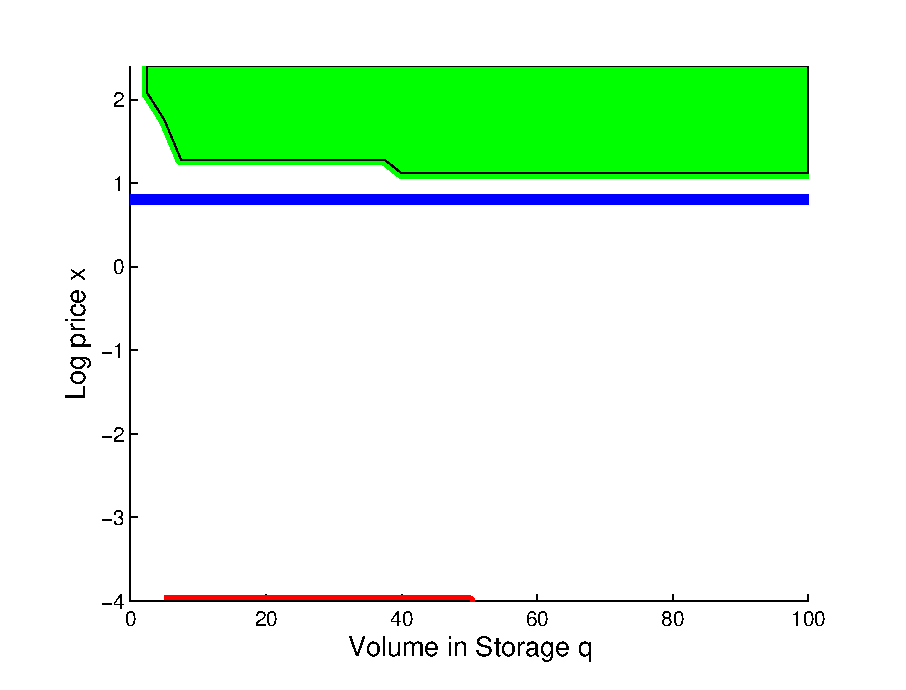
\includegraphics[scale = 0.5]{11step.eps}
%  \caption{11th Step}
%\end{figure}
%}
%
%\only<5>{
%\begin{figure}[hbt]
%  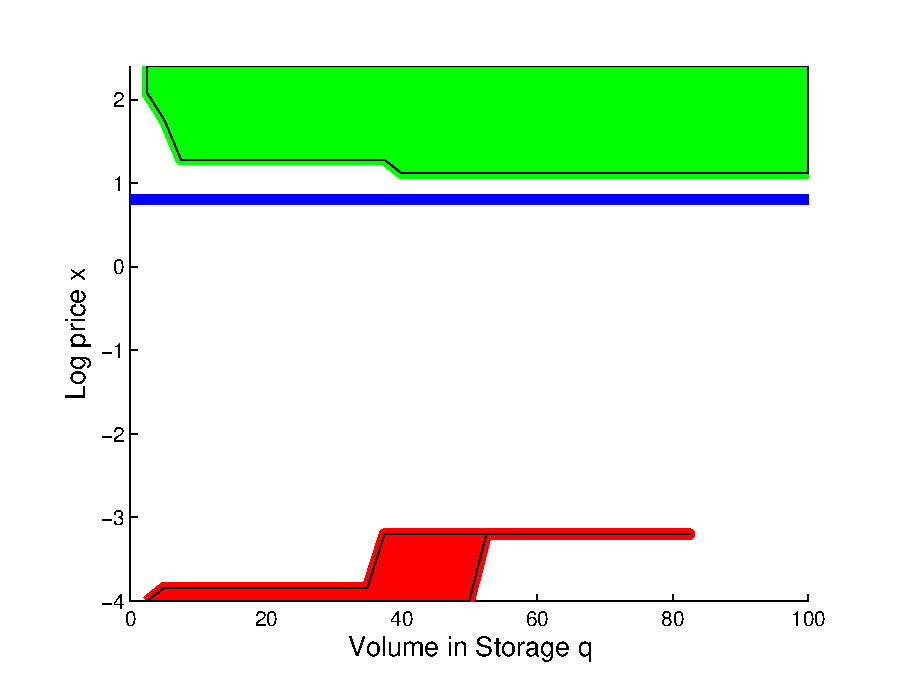
\includegraphics[scale = 0.5]{12step.eps}
%  \caption{12th Step}
%\end{figure}
%}
%
%\only<6>{
%\begin{figure}[hbt]
%  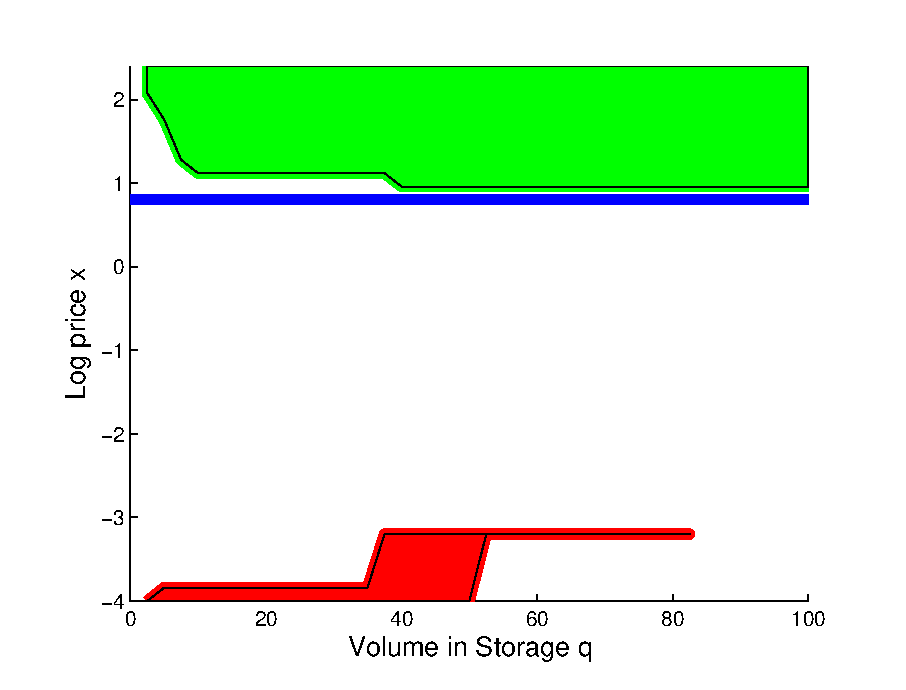
\includegraphics[scale = 0.5]{13step.eps}
%  \caption{13th Step}
%\end{figure}
%}
%
%\only<7>{
%\begin{figure}[hbt]
%  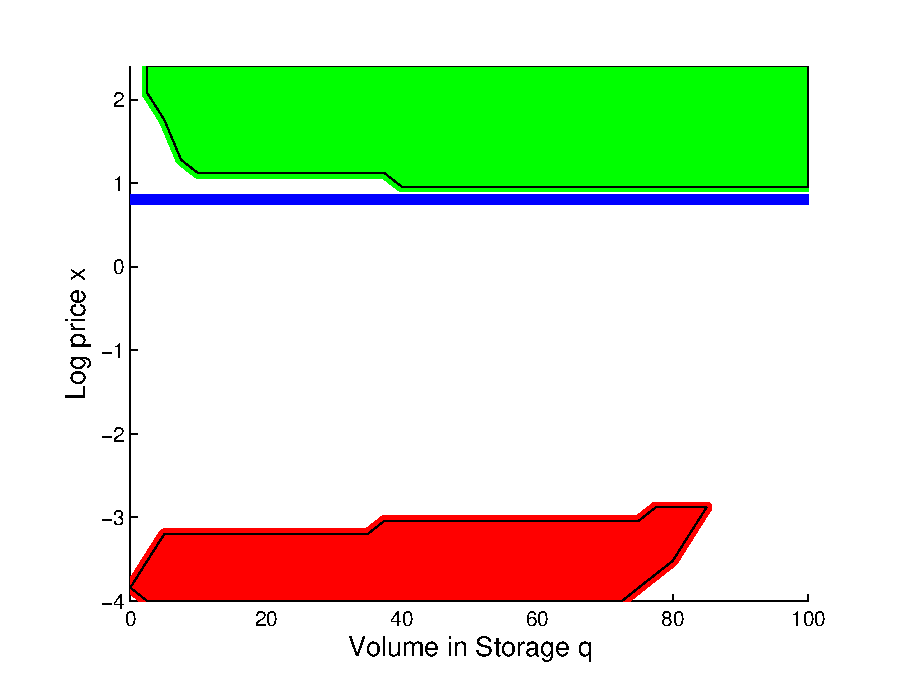
\includegraphics[scale = 0.5]{14step.eps}
%  \caption{14th Step}
%\end{figure}
%}
%
%\only<8>{
%\begin{figure}[hbt]
%  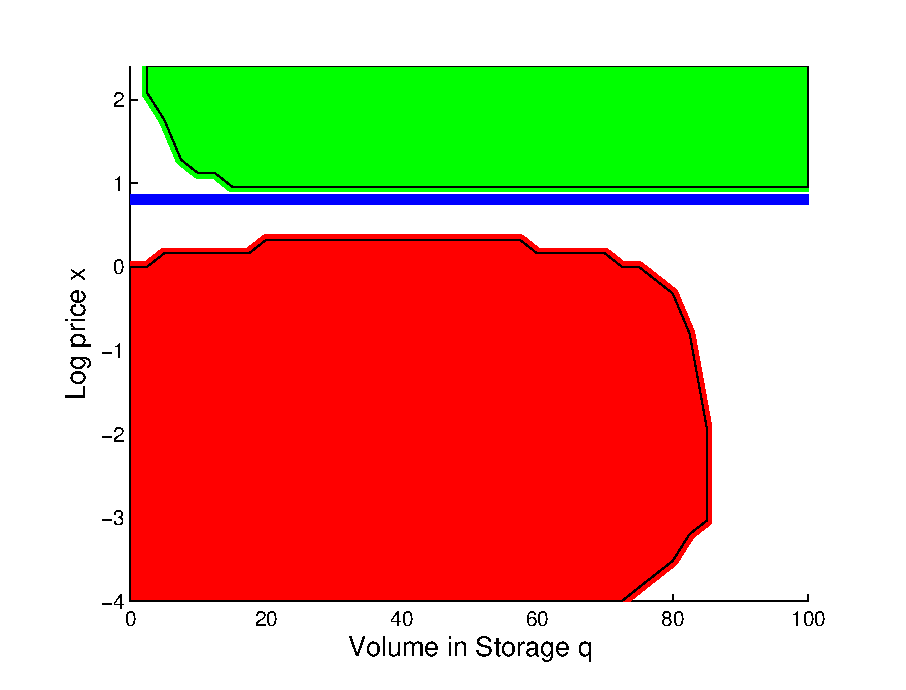
\includegraphics[scale = 0.5]{laststep.eps}
%  \caption{Last Step}
%\end{figure}
%}
%
%\end{frame}

\begin{frame}
{\bf Distance}

{\large Sell}
\begin{columns}
\column{0.5\textwidth}
\only<1>{
\begin{figure}[hbt]
  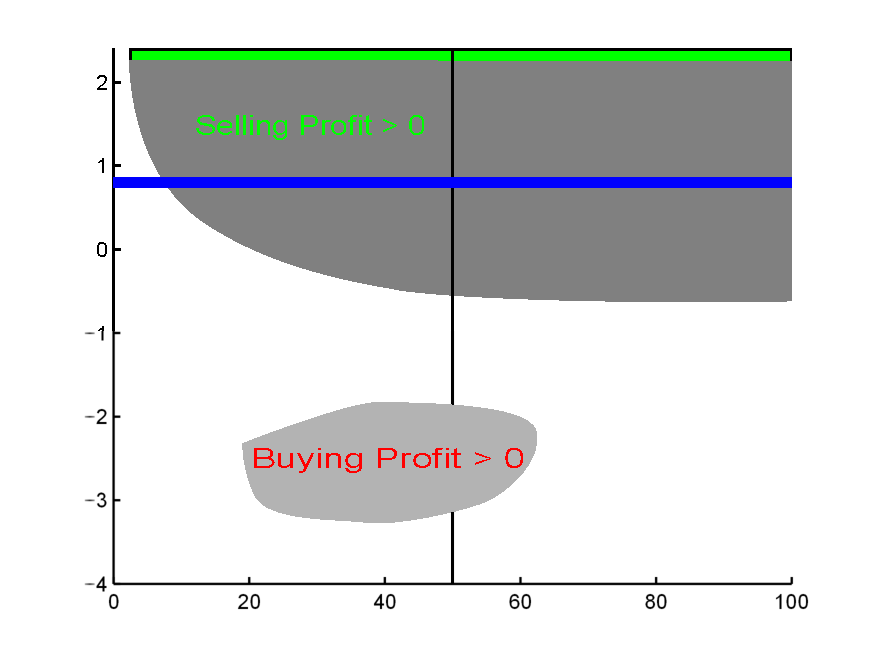
\includegraphics[scale = 0.4]{Where2Move0stepHJBViolation.pdf}
  \caption{Current Policy}
\end{figure}
}
\only<2->{
\begin{figure}[hbt]
  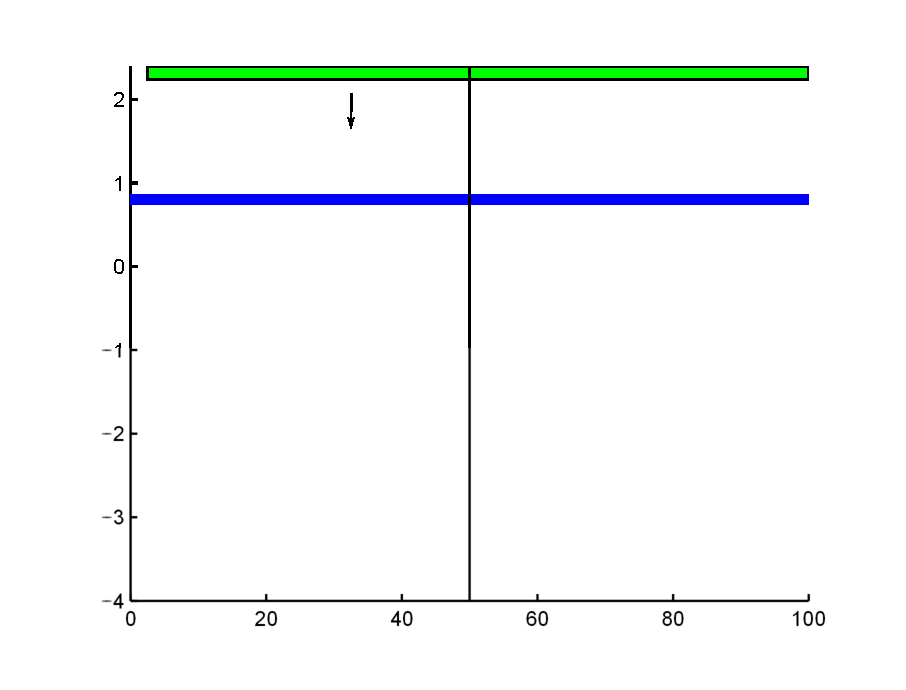
\includegraphics[scale = 0.4]{Where2Move0step.eps}
  \caption{Current Policy}
\end{figure}
}

  \column{0.5\textwidth} 
  \only<2>{
\begin{figure}[hbt]
  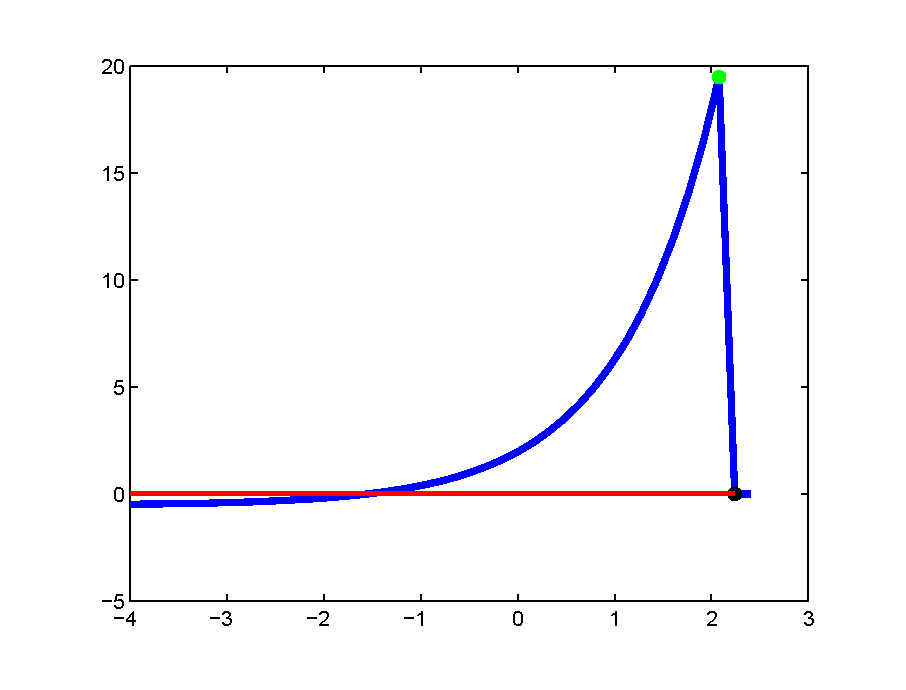
\includegraphics[scale = 0.4]{Where2MoveSell.eps}
  \caption{Selling Profit}
\end{figure}
}
\only<3>{
\begin{figure}[hbt]
  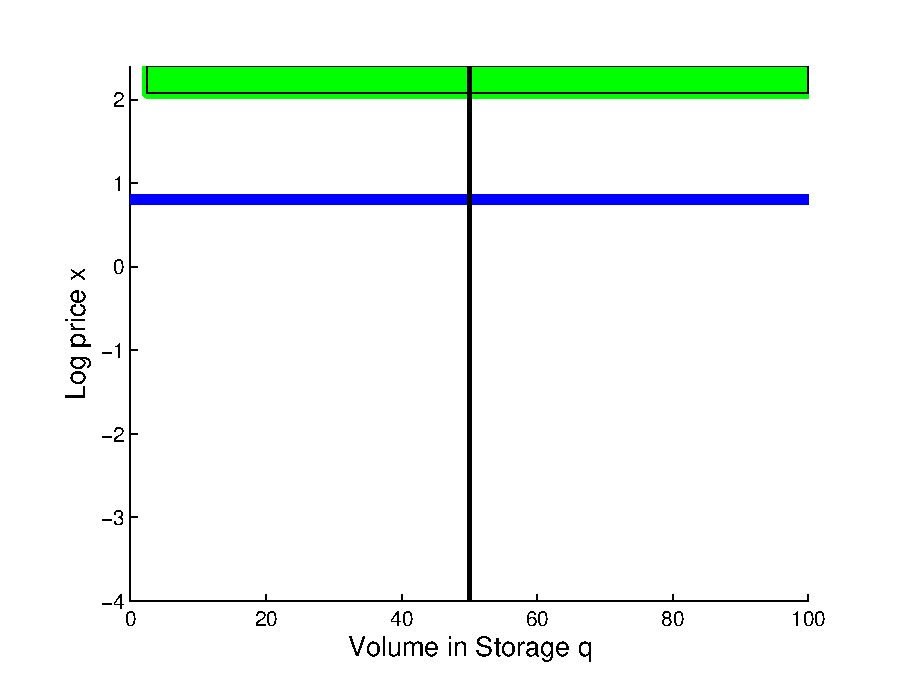
\includegraphics[scale = 0.4]{Where2Move1step.eps}
  \caption{After Movement}
\end{figure}
}
\end{columns}
\end{frame}

\begin{frame}

{\large Buy}
%todo: put a black dot in the graph and an arrow there.
\begin{columns}
\column{0.5\textwidth}
%\only<1>{
\begin{figure}[hbt]
  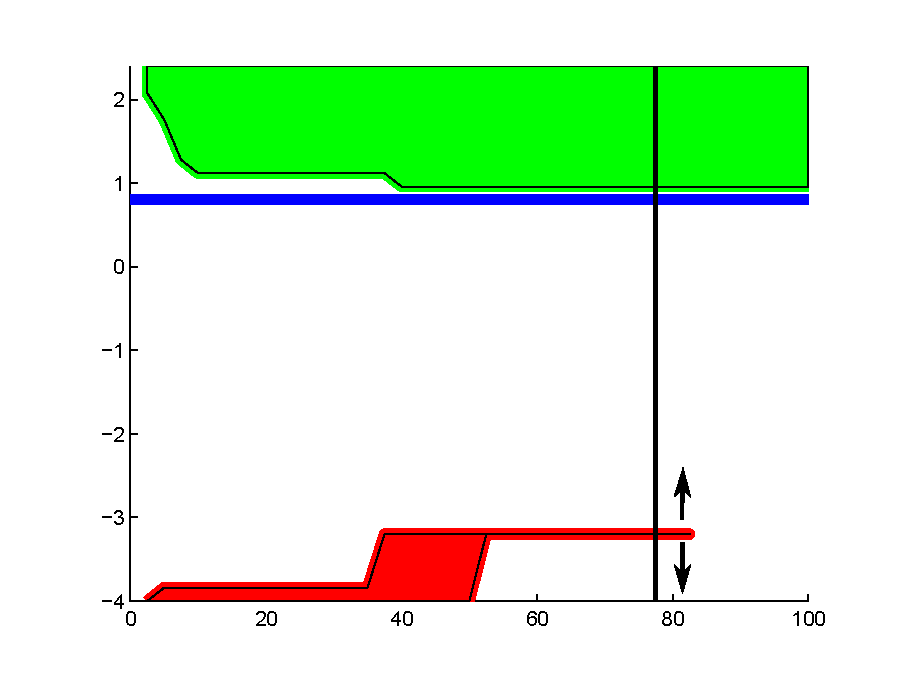
\includegraphics[scale = 0.4]{Where2Move13step.eps}
  \caption{Current Policy}
\end{figure}
%}
  \column{0.5\textwidth} 
\only<2>{
\begin{figure}[hbt]
  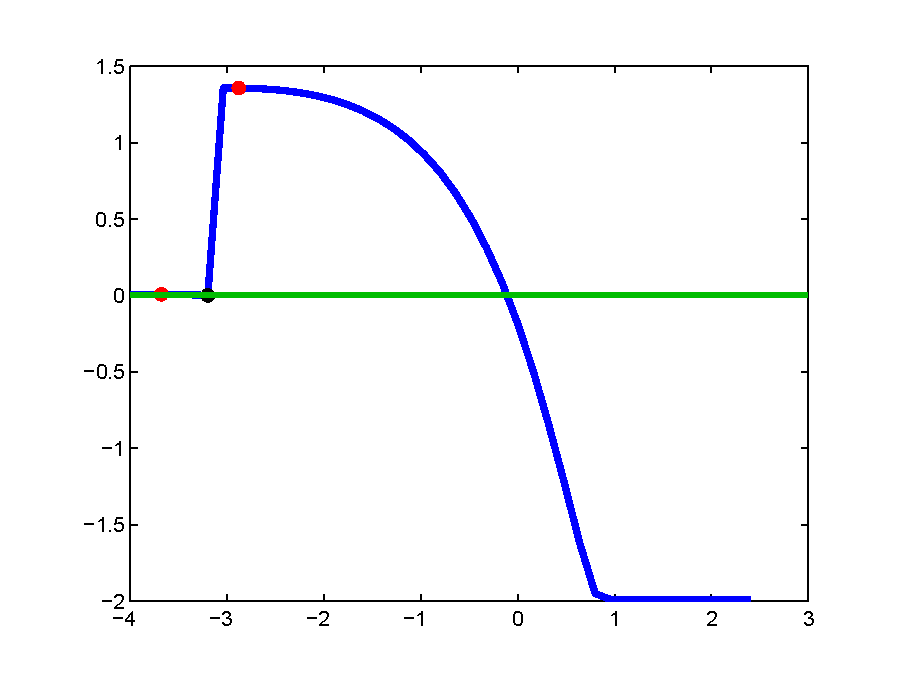
\includegraphics[scale = 0.4]{Where2MoveBuy.eps}
  \caption{Buying Profit}
\end{figure}
}
\only<3>{
\begin{figure}[hbt]
  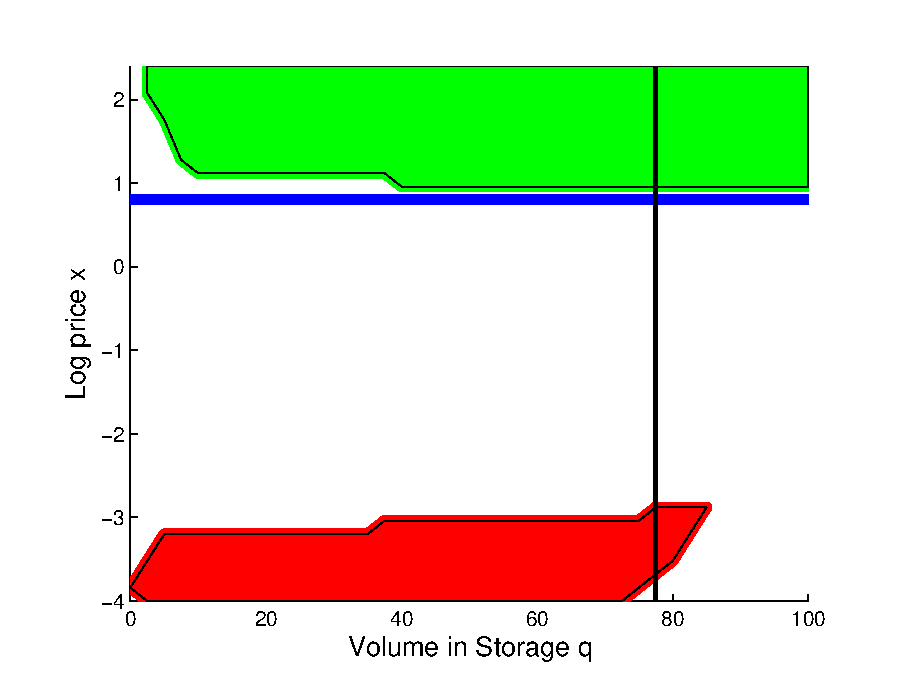
\includegraphics[scale = 0.4]{Where2Move14step.eps}
  \caption{After Movement}
\end{figure}
}
\end{columns}
\end{frame}


\begin{frame}
{\bf Proof of Convergence}
\begin{Theorem}
Each movement improves value function. Namely $\Delta V^{n+1} = V^{n+1} - V^{n}\geq 0 $.
\end{Theorem}

\begin{columns}
\column{0.5\textwidth}
\only<1-2>{
\begin{figure}[hbt]
  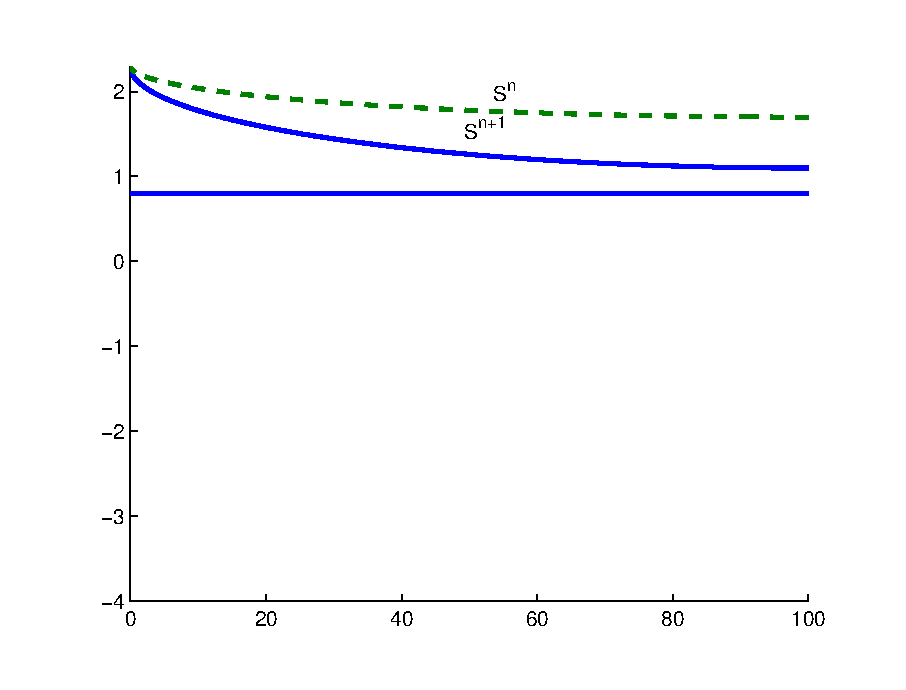
\includegraphics[scale = 0.4]{ProofKeepMoveBoundaries.eps}
\end{figure}
}
\only<3-4>{
\begin{figure}[hbt]
  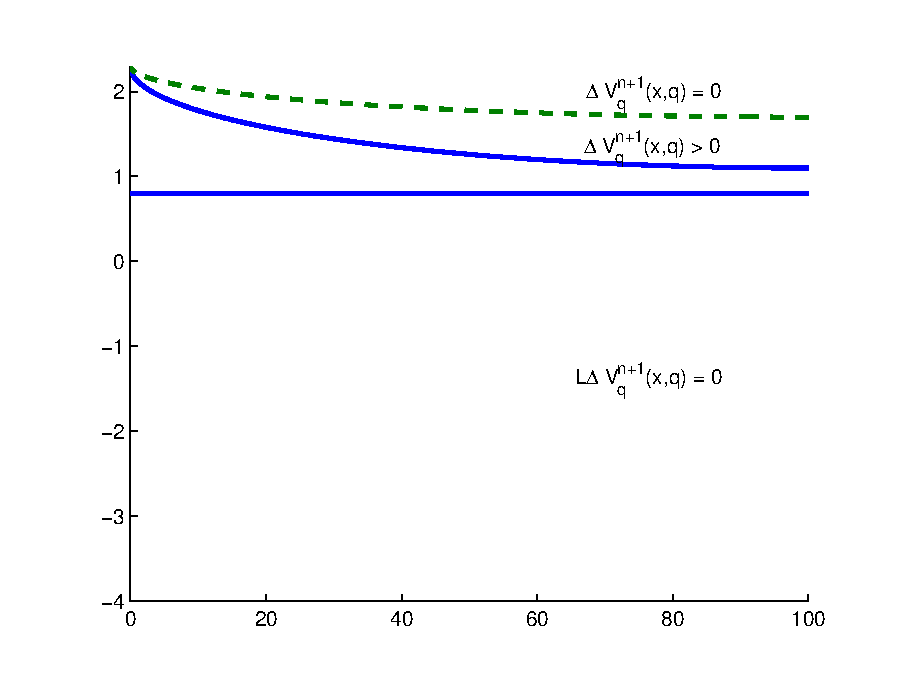
\includegraphics[scale = 0.4]{ProofKeepMoveEquations2.eps}
\end{figure}
}
  \column{0.5\textwidth} 
\only<2-3>{
\begin{figure}[hbt]
  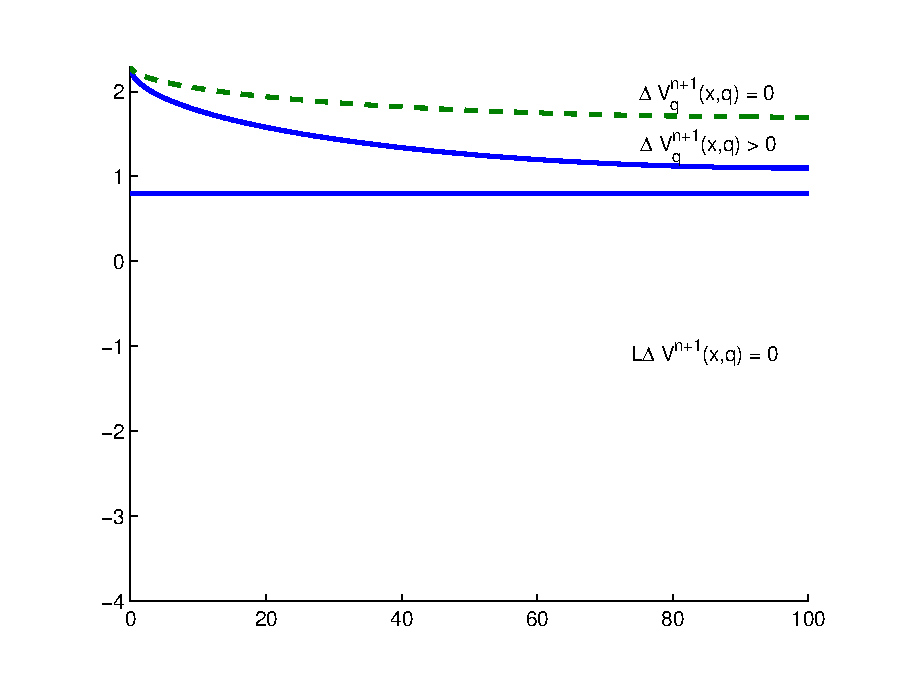
\includegraphics[scale = 0.4]{ProofKeepMoveEquations1.eps}
\end{figure}
}

\only<4>{
\begin{itemize}
  \item $\mathcal{L} \Delta V^{n+1}(x,0) = 0 ~\forall x \in \mathbb{R}$.\\
$\Rightarrow \Delta V^{n+1}(x,0) = 0$.
  \item $\mathcal{L}V = \frac{1}{2} \sigma^2 \frac{\partial^2 V}{\partial x^2} + \alpha (\kappa - x) \frac{\partial V}{\partial x} - \beta V$
Maximum Principle $\Rightarrow \Delta V^{n+1}_q(x,q) \geq 0 $

\end{itemize}



}

\end{columns}

\end{frame}


\begin{frame}
{\bf Proof of Convergence}
% What does \Delta V_q > 0 mean?
\begin{Theorem}
The boundaries can be kept moving. 
\end{Theorem}
\begin{proof}
\begin{equation*}
\begin{split} 
&\Leftrightarrow \left(-V_q^{n+1}(x,q) + (e^x - \mu(q)\right)_x|_{S^{n+1}} < 0\\ 
&\Leftrightarrow \left(-V_q^{n+1}(x,q) + e^x \right)_x|_{S^{n+1}} < 0\\
&\Leftrightarrow \left(-V_q^{n+1}(x,q) + V_q^{n}(x,q) \right)_x|_{S^{n+1}} < 0\\
&\Leftrightarrow \left(\Delta V_q^{n+1}(x,q)\right)_x|_{S^{n+1}} > 0\\
\end{split}
\end{equation*}


\end{proof}




\end{frame}




\begin{frame}
{\bf Extensions}

\begin{itemize}
  \item Seasonality and Finite time.
  \item Depreciation.
  \item Random injection and withdrawal.
  \item Buying and selling price follows different but related stochastic processes. 
\end{itemize}

\end{frame}




\end{document} 